%!TEX TS-program = xelatex
%!TEX encoding = UTF-8 Unicode

\documentclass[12pt]{report}

\usepackage{tocloft}

%\setlength\cftparskip{-2pt}
%\setlength\cftbeforechapskip{0pt}

\usepackage{xecyr}
\usepackage[utf8x]{inputenc}
\usepackage[russian]{babel}

%\usepackage[utf8x]{inputenc}
%\usepackage[english,russian]{babel}

\usepackage[top=2.5cm, bottom=2.5cm, left=3cm, right=2.5cm]{geometry}
% See geometry.pdf to learn the layout options. There are lots.
\geometry{a4paper}                   % ... or a4paper or a5paper or ... 
%\geometry{landscape}                % Activate for for rotated page geometry
%\usepackage[parfill]{parskip}    % Activate to begin paragraphs with an empty line rather than an indent
\usepackage{graphicx}
%\usepackage{amssymb}

\usepackage{fancyhdr}
\pagestyle{fancy}
\lhead{}
\rhead{\footnotesize{Система слежения за лицом человека}}
\cfoot{}
\rfoot{\thepage}

\pagenumbering{arabic}

\usepackage{setspace}
\onehalfspacing

\usepackage{fontspec,xltxtra,xunicode}
\defaultfontfeatures{Mapping=tex-text}
\setromanfont[Mapping=tex-text]{Times New Roman}
\setsansfont[Scale=MatchLowercase,Mapping=tex-text]{Gill Sans}
\setmonofont[Scale=MatchLowercase]{Andale Mono}

% Will Robertson's fontspec.sty can be used to simplify font choices.
% To experiment, open /Applications/Font Book to examine the fonts provided on Mac OS X,
% and change "Hoefler Text" to any of these choices.


\setlength{\parindent}{0cm}
\setlength{\parskip}{12pt plus 0.5ex minus 0.2ex}
\renewcommand{\headrulewidth}{0pt}

%\title{Искусственный интеллект в играх на примере игры "Войны планет"}
%\author{Александр Мочёнов}
%\date{26 Октября 2010 г.}                                           
% Activate to display a given date or no date

\usepackage[largestsep]{titlesec}
\titleformat{\chapter}[hang]{\bf\normalsize\uppercase}{\thechapter}{2pc}{}
\titleformat{\section}[hang]{\bf\normalsize}{\thesection}{2pc}{}	
\titleformat{\subsection}[hang]{\bf\normalsize}{\thesubsection}{2pc}{}
\titlespacing{\chapter}{0pt}{0pt}{0pt}
\titlespacing{\section}{0pt}{*2}{1pt}
\titlespacing{\subsection}{0pt}{*2}{1pt}
\titlespacing{\subsubsection}{0pt}{0pt}{0pt}

\usepackage{hyperref} 
%\usepackage{graphicx}
\usepackage{pstricks}
%\DeclareGraphicsExtensions{.png}

%\newcommand{\executeiffilenewer}[3]{%
% \ifnum\pdfstrcmp{\pdffilemoddate{#1}}%
% {\pdffilemoddate{#2}} >0 {\immediate\write18{#3}}\fi%
%}
%
%\newcommand{\includesvg}[1]{%
%\executeiffilenewer{#1.svg}{#1.pdf}%
%{inkscape -z -D --file=#1.svg --export-pdf=#1.pdf --export-latex}%
%\input{#1.tex}%
%}
\usepackage{subfig}

\usepackage{url}

\usepackage{natbib}
\bibpunct{(}{)}{;}{a}{,}{,}

\usepackage{enumitem}
\newenvironment{myItemize}{
 	\vspace{-10pt}
	\begin{itemize}[nolistsep]
}{\end{itemize}}

\newenvironment{myEnumerate}{
	\vspace{-10pt}
	\begin{enumerate}[nolistsep]
}{\end{enumerate}}

\def\imagetop#1{\vtop{\null\hbox{#1}}}

\usepackage{totcount}
\regtotcounter{figure}
\regtotcounter{table}
\regtotcounter{chapter}

\usepackage[acronym,toc]{glossaries}
\makeglossaries
%\input{glossary}


\renewcommand{\cfttoctitlefont}{\normalsize\textbf}
\setlength{\cftaftertoctitleskip}{18pt}


\usepackage{listings}
\usepackage{algorithm,algorithmic}
\usepackage{multirow}

\usepackage{float}
\floatname{algorithm}{Алгоритм}
\newcommand{\algorithmname}{Алгоритм}

\begin{document}
%\renewcommand{\chaptername}{} 
%\renewcommand{\thechapter}{} 
%\renewcommand{\thesection}{\arabic{section}} 

\begin{titlepage}
  \begin{center}
	\uppercase{Eesti Ettev\~{o}tlusk\~{o}rgkool Mainor}\\*
	Институт инфотехнологии\\*
	Веб программирование\\[8cm]
	Александр Мочёнов\\[1.5cm]
	\large
	\textbf{Метод обнаружения и слежения за положением лица человека на основе нейронных сетей и 
сегментации по цвету кожного покрова}\\[1cm]
	\normalsize
	Дипломная работа\\[2cm]
	\begin{flushright}
		Руководитель: Jelena Faronova, MSc\\[6cm]
	\end{flushright}
	Таллинн 2010
  \end{center}
  
Декларирую, что составил настоящую
дипломную работу самостоятельно.
На все использованные при составлении
работы исследования других авторов,
принципиальные точки зрения,
полученные из литературных источников,
данные, имеются ссылки.
\\[2cm]
\begin{flushright}
``...''........................ 200....г.

Александр Мочёнов
\end{flushright}

\end{titlepage}

\tableofcontents{\thispagestyle{fancyplain}}

\chapter*{Резюме}
%\addcontentsline{toc}{chapter}{Резюме}
\thispagestyle{fancy}

Тема работы: ``Метод обнаружения и слежения за положением лица человека на основе нейронных сетей и 
сегментации по цвету кожного покрова''.

Область компьютерной науки науки, занимающаяся компьютерным зрением стремительно развивается и повсеместно 
применяется. Одной из наиболее популярных направлений в области компьютерного зрения является способность 
распознавать объекты. Частным объектом распознавания является лицо человека. Но для того, что бы его распознать его 
сперва необходимо обнаружить. Этому посвящена данная работа.

Цель автора работы создание системы, которая на практике применяет обнаружение лица человека. В частности создать 
систему умеющую обнаруживать лицо человека с видеокамеры, прикреплённой к сервоприводам и поворачивать в след за 
лицом.

%задачи
Данная работа состоит из 3 основных частей, не включая введение и заключение. В первой части ``введение в 
предметную область'' рассматриваются общие вопросы связанные с компьютерным зрение, распознаванием и обнаружением. 
Так же в этой главе рассматриваются существующие методы и подходы к решению задач, схожих тем, что стоят в данной 
работе. Во-второй главе ``Предлагаемый метод решения '' содержаться описания методов решений всех частей системы. В 
последней главе ``Результаты испытания'' приводятся результаты работы всех частей системы, и приводятся 
рекомендации по улучшению.

TODO Результаты работы.

В работе находиться 25 рисунков.

Ключевые слова: компьютерное зрение, обнаружение лица, искусственные нейронные сети

Работа основана на 28 источниках.

\chapter*{Resume}
%\addcontentsline{toc}{chapter}{Resume}
\thispagestyle{fancy}

R \& D: ``The method of detecting and tracking the position of a person's face based on neural networks and
Segmentation by color of skin.''

Computer science science dealing with computer zraniem rapidly developing and widely primeniyaetsya. One of the 
most popular destinations in the area of ​​computer vision is the ability to recognize the objects. Private object 
recognizers is the person's face. But for the fact that it would recognize it at first to be detected. This paper 
is devoted.

The aim of the author of a system that actually follow the discovery of a human face. In particular, a system able 
to detect a person's face with a webcam attached to the servos and turn in the trail of the person.

% Problem
This work consists of 3 main parts, not including the introduction and conclusion. In the first part of the `` 
Introduction''in the subject area addresses the general issues svzyannye with computer vision, recognition and 
detection. Also in this chapter discusses the methods and approaches to solving problems like the ones that are in 
the work of Dana. In the second chapter, `` The method proposed solutions''include descriptions of methods of 
making all parts of the system. In the last chapter of `` The test results''are the work of all parts of the system 
and resulting recommendations for improvement.

We are 25 resunkov.

Keywords: computer vision, face detection, artificial neural networks

The work is based on 28 sources.

%TODO:

%\printglossary[title=Терминалогия и переводы,style=fancy,toctitle=Терминалогия и переводы]

\chapter*{Введение}
\addcontentsline{toc}{chapter}{Введение}
\thispagestyle{fancy}

Роботы в различных вариациях являются частью жизни человека. Робототехника уже
давно применяются, например, в индустриальном производстве, в детских игрушках,
авиации и многих других местах. Так же роботы применяются в военном деле (беспилотные
самолёты, роботы-сапёры), медицине и даже в космосе\footnote{\url{http://robonaut.jsc.nasa.gov/default.asp}}.

Тем не менее, применение роботов в сфере обслуживания сегодня не так распространено. Оно находится на рубеже науки 
робототехники и пока ещё широко не применяется. В данной работе автор разрабатывает небольшую
часть робота, функционирующего в сфере обслуживания, главной целью которого
является общение с человеком. 

Цель автора данной работы - создать интерактивную систему слежения за человеческим лицом подобием головы робота, 
которая оборудована веб-камерами на месте глаз и сервоприводами, способными поворачивать её по двум осям. Вся 
система состоит из трёх модулей:
\begin{myItemize}
\item Нахождение местоположения и размеры лиц людей на изображении с веб-камеры
\item Выбор лица из найденных, за которым необходимо следовать
\item Вычисление вектора движения и само общение с сервоприводами
\end{myItemize}

Самой сложной из задач является поиск лица человека. В работе автор предлагает последовательный алгоритм, 
который состоит из трёх подзадач, где результат предыдущей является источником данных для последующего:
\begin{myItemize}
\item Предварительная обработка и подготовка изображения;
\item Поиск, сегментация и кластеризация участков кадра, в которых высока вероятность обнаружения лица;
\item Применение искусственных нейронных сетей для окончательной классификации (лицо или нет) по нескольким 
представлениям данного изображения;
\end{myItemize}

%TODO: Почему именно такой?

%TODO: Про real-time сюда?

Подобная система может применяться в любых роботах, обладающих подобием головы.
Например: робот-консьерж в отеле, робот-официант или робот-домохозяйка. Это может упростить и улучшить
впечатление от общения человека с машиной. 
%Так же полученный метод обнаружения лица человека, в случае хороших показателей, можно использовать и в других 
приложениях.

Данная работа состоит из 3 основных частей, не включая введение и заключение. В первой части ``Введение в 
предметную область'' рассматриваются общие вопросы связанные с компьютерным зрением. Приводяться примеры его 
использования, а так же примеры некоторых конкретных проблем, которые решают компьютерное зрение, а именно 
распознавание и обнаружение объектов. Так же в этой главе рассматриваются существующие методы и подходы к решению 
задач, схожих тем, что стоят в данной работе, а именно: методы коммуникации человека и компьютера, методы поиска 
облостей с цветом кожи и методы классификации. 

Во-второй главе ``Предлагаемый метод решения'' содержаться описания методов решения всех описанных частей системы: 
предварительная обработка и подготовка изображения, поиск областей с цветом кожи, классификация и обнаружение лиц и 
выбор лиц для слежения.

В последней, третьей главе ``Результаты испытания'' приводятся результаты работы всех частей системы, из которых 
следует, что алгоритм автокоррекции контраста чёрно-белых изображений работает безупречно и выполняет поставленную 
задачу, а автокоррекция баланса белого работает в пределах нормы, т.к. допускает ошибки. Результат работы 
классификатора в виде искусственной нейронной сети на данном этапе не удовлетворяет потребностям основной 
поставленной задачи. Исходя из результатов по всем задачам приводятся рекомендации по улучшению показателей. 

\chapter{Введение в предметную область}
\thispagestyle{fancy}

%(Про Computer Vision в целом.)
\section{Компьютерное зрение}

Основной частью данной работы является обработка изображений поступающих с веб-камеры. Трансформация данных с видео 
камеры или из статичных изображений в новое представление или принимаемое решение называется - \emph{Компьютерным 
Зрением} (\textit{Computer Vision} или \textit{CV})\citep{bradski2008learning} Т.е. программы и алгоритмы, которые 
в 
своей работе используют визуальную информацию - всё это называют компьютерное зрение.

Человеку, в силу своей зрительной природы, может показаться, что обработка визуальной информации - это очень 
просто, 
но это представление крайне ошибочно. Наш мозг разделяет визуальную информацию на множество каналов, в которых 
зашифрованы различные виды информации, после чего посылает её в мозг человека. В мозгу есть системы распределения 
внимания, в 
ходе работы которой, часть информации обрабатывается, а часть остаётся незамеченной. \citep{bradski2008learning} 
Даже 
сетчатка глаза (внутренняя поверхность глаза, заполненная светочувствительными клетками: колбочками и палочками), 
отвечает за предварительную обработку сигнала. На поверхности сетчатки глаза около 130 миллионов 
светочувствительных 
элементов, а нервных окончаний идущих к мозгу в 100 раз меньше. Это говорит о том, что сетчатка сжимает информацию 
перед отправкой в мозг. В 
частности одной из её функций является \emph{обнаружение границ} (\textit{edge detection}) \citep{RetinaOnWiki}

А что ``видит'' компьютер? Матрицу из чисел, представляющих собой интенсивность света в разных участках 
светочувствительной матрицы. При этом каждая ячейка этой матрицы кроме полезной информации содержит ещё и много 
шума. И в 
этом наборе чисел программа должна найти машину или, например, идущего человека.

%Где и зачем применяется face detection?
Компьютерное зрение широко применяется в медицине, астрономии, метеорологии и других областях науки, где оно 
помогает человеку анализировать и автоматизировать процессы по обработке визуальных данных. 
Например, помогает по снимку с МРТ\footnote{Магнитно-резонансная томограф} указать на опухоль (рис. \ref{fig:mri}) 
или 
анализировать активность клеток крови (рис. \ref{fig:blood_cells}). Подобные задачи называются \emph{распознаванием 
образов} 
(\textit{pattern recognition}). Распознавать можно так же и другие объекты и образы. Например, система 
автоматического 
замера скорости на дорогах распознаёт автомобили и их регистрационные номера, система безопасности следит за
передвижением людей (рис. \ref{fig:track_people}), а в аэропортах и на границе происходит контроль запрещённые 
объекты в багаже (рис. \ref{fig:piston}).

\begin{figure}[h]
	\centering
	\subfloat[]{
		\label{fig:mri}
		\includegraphics[width=0.24\textwidth]{Pictures/kwock3}}
%	\hspace{0.1cm}
	\subfloat[]{
		\label{fig:blood_cells}
		\includegraphics[width=0.24\textwidth]{Pictures/celltracking}}
%	\hspace{0.1cm}
	\subfloat[]{
		\label{fig:piston}
		\includegraphics[width=0.24\textwidth]{Pictures/3d_sift_crop}}
%	\hspace{0.1cm}
	\subfloat[]{
		\label{fig:track_people}
		\includegraphics[width=0.24\textwidth]{Pictures/Reading_People_Tracker_crop}}		
		
	\caption{Примеры применения компьютерного зрения: \subref{fig:mri} обозначенная опухоль на снимке с МРТ, 
\subref
{fig:blood_cells} анализ клеток с помощью CV, \subref{fig:piston} определение запрещённых предметов, \subref
{fig:track_people} слежение за людьми службой безопасности}
	\label{fig:cv_usage}
\end{figure}

%Про Machine Learning в целом?

\emph{Распознавание лица} (\textit{face recognition}) человека является одной из наиболее популярных задач в 
области 
компьютерного зрения. Она заключается в обнаружение и определении по изображению кому именно это лицо принадлежит. 
Решения этой проблемы применяются в системах безопасности (авторизация) и системах управления базами данных лиц 
людей. %TODO More Use cases
С быстрым развитием все более совершенных методов в этой области, распознавание лица человека, как средство 
авторизации, 
представляет из себя более дешёвое решение по сравнению с системами распознавания сетчатки глаза или отпечатка 
пальца. \citep{kumar2006efficient}

К примеру, в популярной программе для работы с цифровыми фотографиями Picasa (\url{http://picasa.google.com/}) есть 
эффективная 
система распознавания, маркировки и каталогизированния найденных на фотографиях лиц людей (рис. \ref{fig:picasa}). 

\begin{figure}[h]
	\centering
	\includegraphics[width=0.5\textwidth]{Pictures/picasa}
	\caption{Интерфейс программы Google Picasa с частью списка найденных на фотографиях лиц.}
	\label{fig:picasa}
\end{figure}

\section{Распознавание и обнаружение лиц}

Но для того, что бы распознать лицо, сначала необходимо найти его место положение и размер на изображении. Эта 
задача называется \emph{обнаружение лица} (\textit{face detection}), что является частным случаем более общей 
проблемы \emph{обнаружения объекта} (\textit{object detection}). Обнаружение лица заключается в том, что бы по 
данному изображению определить, количество, место положения и размеры всех имеющихся лиц. (рис. \ref
{fig:sampledetection}) \citep{liu2010automatically}

\begin{figure}[h]
	\centering
	\includegraphics[width=0.5\textwidth]{Pictures/sampledetection}
	\caption{Обнаружение всех лиц на изображении и обозначение их прямоугольником.}
	\label{fig:sampledetection}
\end{figure}

Почти все алгоритмы распознавания лиц в качестве входных данных используют изображение, содержащее только лицо, 
которое надо распознать. Это изображение можно получить зная его место положенее. По-этому обнаружение лица 
есть предварительная и очень важная задача, которую надо выполнить перед распознаванием. Следовательно от точности 
и 
быстроты определения местоположения лица зависит эффективность всей задачи по распознаванию. 

Но, обнаружение не обязательно должно вести к распознаванию. Обнаружение и слежение за лицом без определения 
принадлежности его к конкретному человеку является основной задачей как данной работы, так и схожих по своей сути 
работ: \citep{capi2010vision}, \citep{luo2007face}, \citep{saxena2008real}.





\section{Существующие методы обнаружения лиц}

Почти все современные подходы к решению задачи обнаружения лица, по мнению автора, содержат так или иначе три 
составляющих:

\begin{description}

%\begin{description}
\item[Подготовка данных]\hfill \\
	Для успешного обнаружения лица поступившие данные необходимо подготовить для дальнейшей работы. Сюда входят и 
различные методы \emph{предварительной обработки} изображения в целом (т.н. \textit{preprocessing}) и методы 
позволяющие уменьшить область поиска или \emph{область интереса} (\textit{region of interest} или \textit{ROI}) для 
ускорения всего процесса обнаружения.
\item[Представление данных]\hfill \\ 
	Изначальное изображение в виде матрицы интенсивностей светочувствительного элемента камеры часто трансформируют 
в 
иные, более компактные отображения или \emph{представления} (\textit{Representation}). Такие изменения чаще всего 
ведут к потере информации, но облегчают процесс классификации.
\item[Классификация]\hfill \\ 
	Само определение наличия или отсутствия в данном участке изображения лица человека. Методов классификации в 
принципе 
(не только лиц) на сегодняшний день существует огромное количество и все они применимы для данной задачи.
\end{description}

\subsection{Методы предварительной подготовки данных}
\subsubsection{Коррекция цвета и освещённости}
\label{sec:preprocessing_theor}
Для эффективной работы с изображением его необходимо подготовить, т.к. бывает, что изображение не контрастно или 
имеет неправильный баланс белого, что может ухудшить процесс обнаружения. Для того, что бы привести изображение в 
порядок применяют различные методы. Некоторые механизмы применяются для всего изображения в целом. Например, 
коррекция контраста и 
баланса белого (рис. \ref{fig:people1}). Другие подготовительные процессы касаются изображений, которые поступают 
непосредственно в классификатор. Речь идёт о небольших частях изображения, которые получаются методов скользящего 
окна (\textit{sliding window}) и масштабирования, которые называют \emph{образцами} %(об этом подробнее в (TODO))
 (см. рис. \ref{fig:sliding_window_method}). 
Процессы коррекции контраста и баланса белого часто накладывают и на образцы (рис \ref{fig:people_faces}), т.к. 
зачастую после исправления контрастности всего изображения, распределение интенсивности в образце всё ещё остаётся 
узким.

\begin{figure}[h]
	\centering
	\subfloat[]{
		\label{fig:people1}
		\includegraphics[width=0.8\textwidth]{Pictures/people.eps}
		}
	\subfloat[]{
		\label{fig:people_faces}
		\includegraphics[width=0.2\textwidth]{Pictures/people_faces.eps}
		}
	\caption{Нормализация всего изображения \subref{fig:people1} и дополнительная нормализация образца \subref
{fig:people_faces}}
	\label{fig:normalize_example}
\end{figure}

В работе \citep{rowley1998neural}, в частности, применяется два метода предварительной обработки образцов. Во-
первых 
производится нелинейное \emph{уравновешивание гистограммы} (\textit{histogram equalization}), которое 
``растягивает'' 
гистограмму (рис. \ref{fig:contrast_norm}), что компенсирует недостающие уровни интенсивности изображения, в 
результате чего изображение становиться 
более контрастным. Во-вторых производиться линейная компенсация интенсивности. Для этого линейная функция 
аппроксимирует общую яркость в каждой из частей образца, после чего она может быть вычтена из образца в случае 
сильной разницы в освещённости разных частей образца. Это приводит к уравновешиванию контрастности в разных частях 
образца (рис. \ref{fig:norm_grad}) 

\begin{figure}[h]
	\centering
	\includegraphics[width=0.5\textwidth]{Pictures/norm_grad.eps}
	\caption{Метод линейной коррекции контрастности. На рисунке сверху оригинальное изображение, ниже результат 
измерения суммарной интенсивности, ниже результат вычитания. \citep{rowley1998neural}}
	\label{fig:norm_grad}
\end{figure}

Похожий алгоритм нормализации интенсивности применяется и в работе \citep{lin2005face}. Перед классификацией каждый 
образец нормализуется по формулам \ref{eq:lin2005_1} и \ref{eq:lin2005_2}.

\begin{equation}
\label{eq:lin2005_1}
\centering
\bar{I}=\frac{1}{N}\sum_{i=1}^{N}I_{i}
\end{equation}
\begin{equation}
\label{eq:lin2005_2}
\centering
{I}'_i=(I_i-\bar{I})+128
\end{equation}

\begin{tabular}{p{3cm} c l}
где & $N$ & -- количество пикселей в образце\\
	& $\bar{I}$ & -- средняя интенсивность по всем пикселям образца\\
	& $I_i$ & -- интенсивность $i$'ого пикселя образца\\
	& ${I}'_i$ & -- нормализованная интенсивность\\
\end{tabular}

Таким образом если какие-то образцы были слишком тёмными или слишком светлыми они все становятся единообразно 
освещены, что упрощает процесс машинного обучения. Пример показан на рисунке \ref{fig:gray_norm}.

\begin{figure}[h]
	\centering
	\includegraphics[width=0.8\textwidth]{Pictures/gray_norm.eps}
	\caption{Применении формул \ref{eq:lin2005_1} и \ref{eq:lin2005_2}.}
	\label{fig:gray_norm}
\end{figure}

Как видно, после преобразования образцы стали однообразны, но при этом в большинстве случаев теряется много 
полезной 
информации. В данной работе применяются схожие методы предварительной обработки образцов и изображения в целом. 
%Подробнее в разделе ....(TODO)

\subsubsection{Сегментация по цвету кожного покрова}
\label{sec:skin_segm}
Чем меньшее изображение необходимо сканировать на наличие лица, тем меньше процессорного времени надо 
затрачивать, что ведёт к ускорению процесса обнаружение. Это можно достигнуть, например, уменьшением всего 
изображения, что 
ведёт к потере разрешающей способности данного подхода. Одним из способов позволяющих уменьшить площадь 
сканирования и одновременно не потерять разрешающей способности является эвристическое знание о том, что все лица 
людей покрыты кожным покровом. Это можно использовать для нахождения областей изображения содержащих цвета схожие с 
цветами кожного покрова (\textit{skin-color detection}), и в дальнейшем осуществлять сканирование только этих 
областей.

Среди методов обнаружения лиц, основанных на поиске признаков (\textit{feature based}), подходы использующие 
информацию 
о цвете кожи, как признак обнаружения, получают всё большую популярность. Цвет легко и быстро обрабатывать и он 
инвариантен к геометрическим особенностям образов лиц людей. К тому же опыт подсказывает, что кожа человека 
имеет отчётливый характерный цвет, который легко узнаваем людьми. \citep{vezhnevets2003survey} Цвет кожи - это один 
из тех признаков, что не зависит от положения лица, частичной закрытости и контраста, по-этому именно этот метод 
часто используют для локализации лиц. \citep{ruangyam2009efficient}

Такой метод возможен благодаря тому факту, что различные цветовые вариации кожных покровов людей (даже среди 
представителей различных этнических групп) лежат в достаточно узком диапазоне и отличаются только яркостью (\textit
{luminance}), в тоже время цветность (\textit{chrominance}) практически не меняется. Цвет кожи лежит в основном в 
красной части цветового спектра и определяется цветом крови. А яркость определяется прозрачностью эпидермиса 
(верхнего слоя кожи), за что в свою очередь отвечает концентрация меланина. \citep{xu2006color} %Подробнее в 
%разделе ... (TODO)

\subsection{Методы представления изображения}
Одно и тоже изображение можно представить разными способами. Это нужно для того, что бы обучаемые классификаторы 
(см. 
\ref{classficators}) могли обучаться на различных характеристиках или признаках, имеющихся в различных 
представлениях. 

\subsubsection{Пиксельная интенсивность}
Самым простым и популярным представлением является информация об интенсивности в каждом пикселе изображения. Такой 
метод представления считается не имеющим потерь (\textit{lossless}). Т.е. в нём присутствует  вся информация об 
оригинальном изображении. \citep{bojkovic2006face} Пример на рисунке \ref{fig:house_gray}.

\subsubsection{Информация о контурах}
Любой метод обнаружения лиц%, в прочем как и все другие алгоритмы в компьютерном зрении,
 должен быть стойким к таким вещам 
как поза головы, угол обзора, освещение и многим другим факторам. 

Для решения проблемы с освещением используется \emph{информация о контурах} (\textit{edginess}) или \emph{градиент 
изображения}. Одно и то же лицо под разными источниками света с точки зрения пиксельного представления совершенно 
отличны друг от друга, что создаёт проблему для классификатора найти среди них нечто общее. С другой стороны 
информация о пограничных областях в большей степени неизменна. \citep{ahmadyfard2008hierarchical}

Это представление, в отличая от пиксельного представления, не содержит всей изначальной информации. Сохраняется 
информация лишь о пограничных контрастных зонах лица (глаза, брови, губы). Пример такого представления на рисунке 
\ref{fig:house_gray_sobel}.

\subsubsection{Собственные лица}
\emph{Собственное лицо} (\textit{eigenface}) - это набор \emph{собственных векторов} (\textit{eigen vectors}), 
используемых для описания ``стандартизированных  компонентов лица''. Один образец лица принимается как точка в 
многомерном пространстве. Много образцов образуют компактную область в этом пространстве. Задача заключается в 
нахождении 
\emph{главных компонент} (\textit{principal components}) этой области, параметрами которых её можно описать, 
используя значительно меньшее количество переменных, нежели для описания всех точек изначального пространства.
\citep{turk1991eigenfaces}

Собственный вектор представляет из себя набор параметров, которыми можно описать ``среднестатистическое'' лицо 
человека. Их же можно хранить, например, в базе данных, или использовать в качестве представления группы 
изображений. Этот набор параметров является своего рода выжимкой из многих тренировочных лиц и может использоваться 
для дальнейшей классификации. Эти параметры можно спроецировать в виде изображения. Примеры собственных лиц 
приведены на рисунке \ref{fig:eigenfaces}.

В работе \citep{tsai2006face} автор в процессе обнаружения лиц использует собственные лица для поиска областей-
кандидатов на наличие лицам, а нейронная сеть проводит конечную классификацию.

\begin{figure}[h]
	\centering
	\subfloat[]{
		\label{fig:house_gray}
		\includegraphics[width=0.3\textwidth]{Pictures/dr_house_gray.png}
		}
	\subfloat[]{
		\label{fig:house_gray_sobel}
		\includegraphics[width=0.3\textwidth]{Pictures/dr_house_gray_sobel.png}
		}
	\subfloat[]{
		\label{fig:eigenfaces}
		\includegraphics[width=0.35\textwidth]{Pictures/eigenfaces.jpg}
		}
	\caption{Различные представления изображений: \subref{fig:house_gray} обычное пиксельное представление, \subref
{fig:house_gray_sobel} нормализованный Собелев градиент по $y$, \subref{fig:eigenfaces} набор из различных 
собственных лиц}
	\label{fig:representations}
\end{figure}

\subsubsection{Характеристики типа Хаара}
\emph{Характеристики типа Хаара} (\textit{Haar-like features}) представляют изображения в виде набора характеристик 
полученных вычитанием сумм интенсивностей одних областей из других по определённому шаблону. Это представление 
применяется платформой по обнаружению объектов Виола-Джонса (\textit{Viola-Jones object detection 
framework}). \citep{viola2001rapid} Этод метод и применяемое в нём представление является одним из самых быстрых на 
сегодняшний день методов обнаружения объектов.
%Мало, может ещё чего. Подробнее?

\subsubsection{Использование нескольких представлений}
Многие решения обнаружения лиц используют сразу несколько представлений. Это позволяет использовать более широкий 
спектр характеристик, что делает классификатор более чувствительным к особенностям конкретного вида объектам (в 
данном случае к лицам).

Так в работе \citep{bojkovic2006face} используются три представления: пиксельное, коэффициенты собственных лиц и 
профильные коэффициенты. В работе \citep{ahmadyfard2008hierarchical} авторы используют две представления: 
пиксельное и 
информацию о контурах. По их словам ``объединение информации об интенсивности и о контурах даёт более описательные 
характеристики для представления изображения с лицом''.

\subsection{Задача классификации}
\label{classficators}
Задача \emph{классификации} - это проблема определения класса из всех возможных, к которому относятся 
классифицируемые объекты или наблюдения. Классификация тесно связана с \emph{машинным обучением} (\textit{Machine 
Learning} или \textit{ML}), задачей которого является превращение данных в информацию. \citep{bradski2008learning}

Задача обнаружения лица является классическим примером задачи классификации, где есть всего два класса ``лицо'' или 
``не лицо''. Классификатор должен по данному ему изображению уметь определить к какому классу из двух оно 
относиться.

Все методы классификации можно грубо разделить на две части: классификаторы основанные на знаниях (\textit
{knowledge-based}) и 
статистически обучаемые. Основанные на знаниях используют эмпирические знания о местоположении и распределении 
органических характеристик лица. \citep{bojkovic2006face} Например, что глаза находятся в верхней половине 
картинки и они симметричны, а под ними находиться рот, с которым они образуют равнобедренный треугольник. Такие 
алгоритмы легко реализовать, но они неустойчивы ко многим факторам (например, наклон головы).

К статистически обучаемым алгоритмам классификации относятся те, что получают знания из данных при обучении с 
учителем или без него. Т.е. работа таких алгоритмов состоит из двух этапов: обучение и само использование. Самих 
методов очень много. Ниже приведены те, что чаще всего встречаются в работах по обнаружению лиц. 

\subsubsection{Метод опорных векторов}
\emph{Метод опорных векторов} (\textit{Support vector machine} или \textit{SVM}) заключается в нахождении 
разделяющей 
гиперплоскости в более высокомерном пространстве, чем классифицируемые вектора. Конечная плоскость должна быть 
максимально удалена от представителей разных классов. Для этого находятся наиболее близкие к этой плоскости и тем 
самым более влиятельные векторы, которые называют опорными векторами. \citep{shavers2006svm}

Ограничением SVM подхода является проблематичность использования для классификации более чем по двум классам. 
Впрочем в 
данной задаче речь как раз и идёт о двух классах и SVM хорошо справляется с ней во многих работах. \citep
{shavers2006svm}, \citep{jee2004eye}, \citep{saxena2008real}
%\subsubsection{PCA}
\subsubsection{Искусственные нейронные сети}
Одним из самых популярных (но не самым эффективным) методом классификации до сих пор является искусственные 
нейронные 
сети (далее ИНС, \textit{Artificial Neural Network} или \textit{ANN}). Этот способ применяется в большинстве 
научных 
работ изученных в ходе подготовки данной работы, что стало одним из факторов выбора её в качестве классификатора. 

Появление ИНС было вдохновлено биологическими системами, в частности, нервной системой. До определённой степени 
структура и функциональность ИНС напоминают структуры нейронных связей головного мозга (рис \ref{fig:neurons}). 
Биологический нейрон это - нервная клетка, у которой есть сеть окончаний \emph{дендритов}, через которые она 
получает сигнал от 
других нейронов. В ядре клетки происходит суммирование всех сигналов, после чего он передаётся по длинному 
выходному 
окончанию \emph{аксону} на входы следующих нейронов. В ИНС всё похоже. У нейрона есть входной вектор (сеть 
дендритов), все значения которых умножаются на веса соответствующих связей и суммируются, после чего суммарный 
сигнал 
проходит через \emph{активационную функцию} (ядро) и результат передаётся к последующему нейрону как один из 
компонентов его входного вектора (аксон). 

\begin{figure}[h]
	\centering
	\subfloat[]{
		\label{fig:neuron}
		\includegraphics[width=0.4\textwidth]{Pictures/neuron.jpg}
		}
	\subfloat[]{
		\label{fig:art_neuron}
		\includegraphics[width=0.6\textwidth]{Pictures/art_neuron.png}
		}
	\caption{Биологический \subref{fig:neuron} и искусственный \subref{fig:art_neuron} нейроны. На рисунке \subref
{fig:art_neuron}: $w_{1..i}$ - веса входящих соединений, $1$ - входящий сигнал, $2$ - суммирует входящие взвешенные 
сигналы, $3$ - активационная функция преобразует сумму сигналов, $4$ - результат передаётся на входы других 
нейронов.}
	\label{fig:neurons}
\end{figure}

Определяющими факторами работы ИНС являются: топология или структура сети, виды активационных функций и веса 
соединений. Веса соединений - это параметры сети, они меняются во время обучения сети, после чего сеть может 
описывать модель, которую её учат классифицировать. Главной задачей активационной функции является сжатие сигнала 
до 
определённых границ, а так же усиление слабых сигналов и гашении сильных. Самой популярной функцией является 
сигмовидная. Она обладает всеми описанными выше требованиями к активационной функции и к тому же 
обладает простой производной, что очень удобно во время обучения методом обратного распространения. \citep
{wasserman1989neural}

Концептуально есть две структуры ИНС: с прямым распространением сигнала (\textit{feedforward}) и рекуррентные (т.е. 
с 
обратными связями). Второй тип применяется для обучения без учителя (\textit{unsupervised learning}) и в 
обнаружении 
используется реже, чем первый тип, к которому применяют метод обучения с учителем (\textit{supervised learning}).

Популярным методом обучения ИНС с прямым распространением является алгоритм \emph{обратного распространения ошибки} 
(\textit{backpropagation}) ``Он имеет солидное математическое обоснование. Несмотря на некоторые ограничения, 
процедура обратного распространения сильно расширила область проблем, в которых могут быть использованы 
искусственные 
нейронные сети, и убедительно продемонстрировала свою мощь.'' \citep{wasserman1989neural} Принцип метода такой: 
\begin{myItemize}
\item cначала на вход сети подаётся входной вектор, который проходит через сеть и сеть выдаёт результат;
\item разница полученного результата и заранее известного необходимого выхода (``правильного ответа'') сети 
посылается в обратном направлении от выходов к входам;
\item по мере прохождения высчитывается ошибка по методу наименьших квадратов;
\item по этой ошибке методом \emph{градиентного спуска} высчитываются изменения весов соединений. Таким образом с 
каждым новым образцом веса меняются всё лучше описывая желаемую модель.
\end{myItemize}

 У ИНС метода есть и проблемы. Что бы получить результат выше среднего сеть должна быть очень точно отрегулирована 
(число слоёв, число узлов, скорость обучения и т.д.) \citep{jee2004eye} Авторы работы \citep{capi2010vision} так же 
считают, что эффективность работы зависит от качества подстроки всей системы, и что это трудоёмкая работа. 
Результат 
данной работы лишний раз подтверждает эти выводы.

\section{Вспомогательные методы обнаружения лиц}

На тему обнаружения лиц написано огромное количество научных работ. В базе данных IEEE Xplore за период с 2000 года 
можно найти свыше 6000 работ, так или иначе связанных с данной тематикой. В каждой из них есть какая-то своя, 
оригинальная идея.

Так, в работе \citep{jee2004eye} одной из главных характеристик поиска являются глаза, которые обнаруживаются на 
изображении при помощи SVM классификатора.

В работе \citep{capi2010vision} решается проблема создания навигационной системы робота, способной следовать за 
человеком, используя визуальную информацию. Для этого сначала обнаруживается лицо человека, а после определяется 
основной цвет его одежды. Далее человек может развернуться, и робот будет следовать за ним ориентируясь по одежде, 
а не по лицу.

Похожие задачи стоят в работе \citep{luo2007face}, где решают проблему взаимодействия человека и робота (\textit
{Human-Robot Interaction} или \textit{HRI}). Стоит задача обнаружения лица человека и дальнейшего слежения за ним. 
Особенностью этой работы является способ уменьшения области интереса, в которой высока вероятность обнаружения 
лица. 
Для этого информация о положении лица берётся из предыдущих кадров, высчитывается траектория движения лица и 
прогнозируемое следующее положение, после чего эта область расширяется на константу и в полученном месте 
изображения 
уже производиться поиск лица.

В работе \citep{zhang2010fast} применяется простая идея о том, что лицо человека, как и сама голова, скорее всего в 
кадре будет двигаться. Так областью интереса можно определить все движущиеся объекты. Но, такой метод предполагает 
статичную камеру и следовательно статичный фон.

%(про real-time)

\chapter{Предлагаемый метод решения}
\thispagestyle{fancy}
\section{Концепция решения}
В этой работе предлагается метод состоящий из трёх модулей, которые в совокупности образуют классический \emph
{интеллектуальный агент} (см. \ref{fig:agent}). 

\begin{figure}[h]
	\centering
	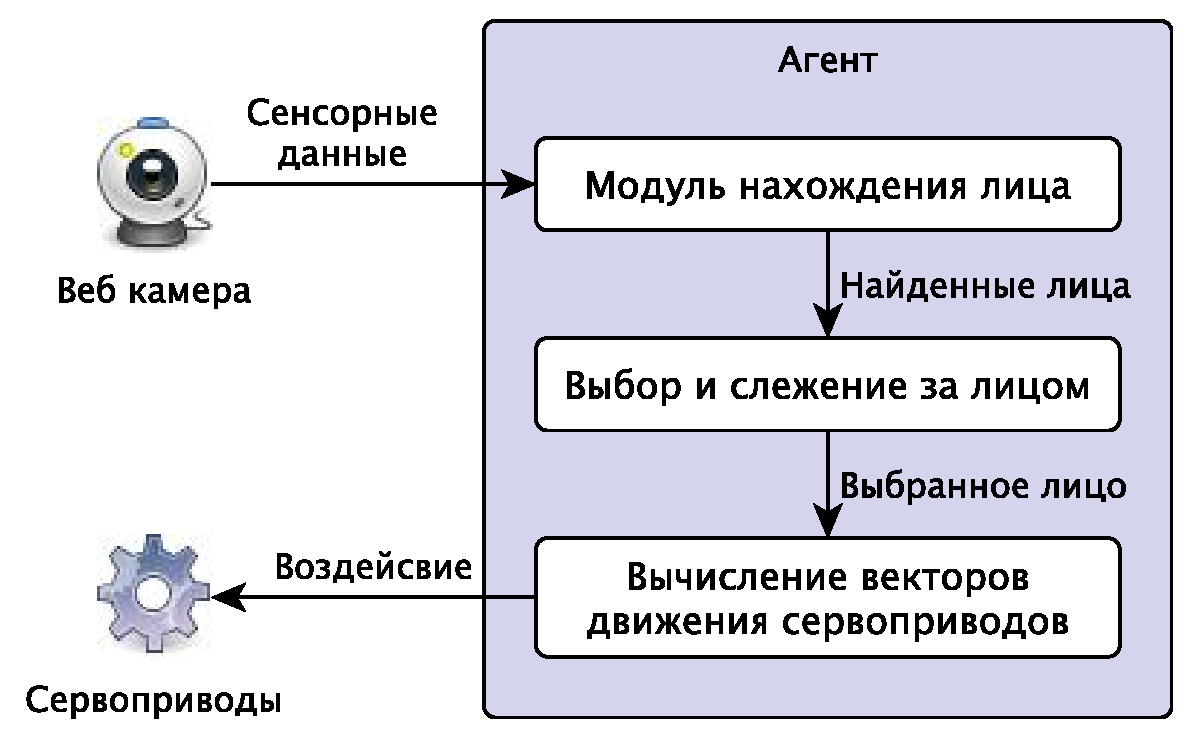
\includegraphics[width=0.6\textwidth]{Pictures/Agent.eps}
	\caption{Высокоуровневая структура всей системы.}
	\label{fig:agent}
\end{figure}

Агент обладает способностью воспринимать окружающую среду через сенсоры, функцию которых выполняет веб-камера. 
После 
обработки полученных данных агент в каком-то роде может воздействовать на среду, вращая сервоприводы. \citep
{рассел2006искусственный}

Информация с веб-камеры поступает в модуль нахождения лиц, откуда данные о найденных лицах поступают в модуль 
выбора 
и слежения. Тут происходит выбор того лица, за которым следить. После выбора модуль работы с сервоприводами даёт 
команду на вращение. Такая модульная структура позволяет в случае необходимости заменить тот или иной модуль. 

В предложенном решении основной программный код написан на языке \textit{Python}. Чтобы не тратить время на 
решение 
уже решённых кем-то проблем, используются следующие программные библиотеки:
\begin{description}
%\begin{description}

\item[OpenCV]\hfill \\
	OpenCV\footnote{Open Source Computer Vision Library. \url{http://opencv.willowgarage.com/}} - самая популярная 
и 
используемая библиотека компьютерного зрения с открытым исходным кодом. Библиотека написана на \textit{С}\textbackslash{}\textit{С++} и работает под \textit{Linux}, \textit{Windows} и \textit{Mac OS X}. Так же разрабатываются интерфейсы 
для языков \textit{Python, Matlab, Ruby, Lua} и других. ``Цель OpenCV - предоставить простую в использовании 
инфраструктуру компьютерного зрения, которая поможет людям строить достаточно сложные приложения.'' \citep
{bradski2008learning}
	
В данной работе используется очень интенсивно для всех манипуляций с изображением.

\item[PyBrain]\hfill \\
	PyBrain\footnote{\textbf{Py}thon-\textbf{B}ased \textbf{R}einforcement Learning, \textbf{A}rtificial \textbf{I}
ntelligence and \textbf{N}eural Network Library. \url{http://pybrain.org/}} - модульная \textit{Python} библиотека 
машинного обучения с открытым исходным кодом. Имеет широкий набор алгоритмов для обучения с учителем, без учителя, 
обучения с подкреплением, оптимизации типа ``чёрный-ящик'' (\textit{black-box optimization}).
	
В данной работе библиотека используется для конструирования, обучения и применения ИНС.

\item[NetworkX]\hfill \\
NetworkX\footnote{\url{http://networkx.lanl.gov/}} - \textit{Python} библиотека для работы с графами. В данной 
работе 
нужна для поиска минимального остовного дерева.

\end{description}

\section{Модуль нахождения лица}

Модуль нахождения лица является самой большой частью данной работы, то есть в нём сосредоточена основная логика всей 
системы. Схематически весь алгоритм представлен на рис. \ref{fig:face_detect_module1}. Каждый подмодуль 
соответствует 
отдельному алгоритму и он будет рассмотрен в данном разделе более подробно. %(TODO Подробнее описать что да как?)

\begin{figure}[h]
	\centering
	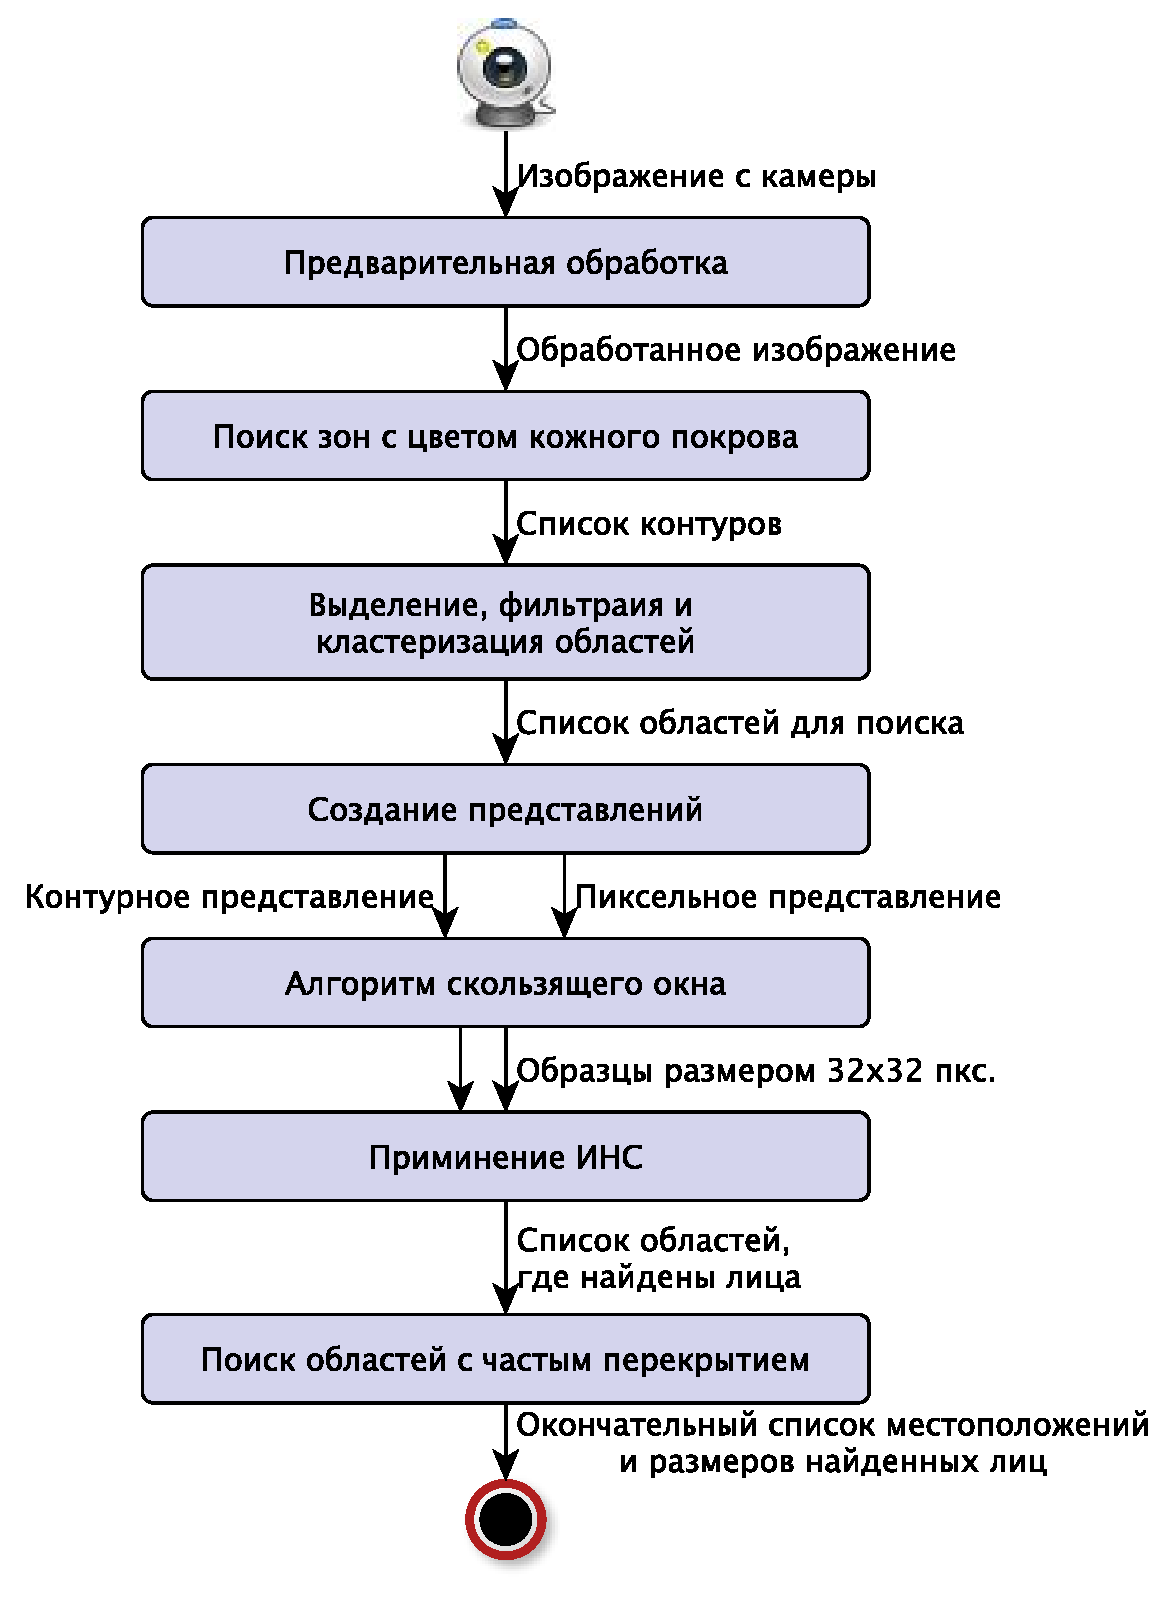
\includegraphics[width=0.7\textwidth]{Pictures/face_detect_module2.eps}
	\caption{Алгоритм обнаружения лиц}
	\label{fig:face_detect_module1}
\end{figure}

\subsection{Предварительная обработка}

В данной работе для подготовки изображения для дальнейшей работы используется метод \emph{нормализации 
гистограмм} каждого из каналов изображения. Необходимость данного этапа приведена в разделе \ref
{sec:preprocessing_theor}. Цель данного этапа получить более контрастную картинку с минимальной потерей информации 
и 
исправление баланса белого.

\subsubsection{Нормализации гистограмм}
\emph{Гистограмма} - это графическое представление, дающее наглядное представление о распределении данных. График состоит 
из 
прямоугольников, которые показывают количество наблюдений (ось ординат) на данном промежутке (ось абсцисс). На 
рисунке \ref{fig:histo_sheldon} показана гистограмма распределения пиксельных интенсивностей данного (\ref
{fig:sheldon})  Ч\textbackslash{}Б изображения. Стоит отметить, что в цветном изображении у каждого цветового 
канала 
своя гистограмма.

\begin{figure}[h]
	\centering
	\subfloat[]{
		\label{fig:sheldon_hist}
		\includegraphics[width=0.35\textwidth]{Pictures/sheldon_hist_255.eps}
		}
	\subfloat[]{
		\label{fig:sheldon}
		\includegraphics[width=0.25\textwidth]{Pictures/sheldon.eps}
		}
	\subfloat[]{
		\label{fig:sheldon_hist_35}
		\includegraphics[width=0.35\textwidth]{Pictures/sheldon_hist_30.eps}
		}
	\caption{Гистограмма распределения интенсивностей пикселей изображения \subref{fig:sheldon}. \subref{fig:sheldon_hist} для каждой интенсивности свой столбец, \subref{fig:sheldon_hist_35} все интенсивности распределены между 30-ью столбцами.}
	\label{fig:histo_sheldon}
\end{figure}

В данном примере по оси абсцисс интервалами являются промежутки возможных интенсивностей. На гистограмме справа 
\subref{fig:sheldon_hist} один промежуток соответствует одному конкретному значению интенсивностей. Для 8-и битного 
Ч\textbackslash{}Б изображения значение может быть от 0 до 255, где 0 - это чёрный, а 255 - белый цвета. На 
гистограмме слева \subref{fig:sheldon_hist_35} показано, что ``столбики'' (\textit{bins}) могут объединять значения 
на равных интервалах , показывая тем самым менее детальное распределение между равными частями всех значений.

В случае изображений с низкой контрастностью рис. \ref{fig:low_contr1} гистограмма ``сжата'' и все значения 
сосредоточены на узком участке возможных интенсивностей рис. \ref{fig:low_contr_hist}. Как видно с гистограммы 
изображение содержит только пиксели средние интенсивности, т.е. серые цвета. По-этому на нём нету ни белого, ни 
чёрного цветов.

\begin{figure}[h]
	\centering
	\subfloat[]{
		\label{fig:low_contr1}
		\includegraphics[width=0.5\textwidth]{Pictures/low_contr_1.jpg}
		}
	\subfloat[]{
		\label{fig:hight_contr}
		\includegraphics[width=0.5\textwidth]{Pictures/low_contr_1_norm.png}
		}
		
	\subfloat[]{
		\label{fig:low_contr_hist}
		\includegraphics[width=0.51\textwidth]{Pictures/x2_b}
		}
	\subfloat[]{
		\label{fig:hight_contr_hist}
		\includegraphics[width=0.5\textwidth]{Pictures/low_contr_1_norm.eps}
		}
	\caption{Нормализация контраста ``растяжением'' гистограммы.}
	\label{fig:contrast_norm}
\end{figure}

Что бы исправить положение и сделать изображение более интенсивным необходимо ``растянуть'' гистограмму (рис. \ref{fig:hight_contr_hist}). Как видно после такого растяжения изображение стало более контрастным, на нём появились более тёмные и светлый цвета 
\ref{fig:hight_contr}. На модифицированной гистограмме видны пробелы, они свидетельствуют о недостаточной информации и 
скачкообразных переходах интенсивностей изображения.

\subsubsection{Баланс белого цвета}

\emph{Баланс белого цвета} (реже \emph{цветовой баланс} от \textit{color balance}) - это показатель нейтральности 
основных цветов (красный, зелёный и голубой) на изображении. Бывают ситуации, когда эта нейтральность нарушена и на 
изображении превалирует какой-то из цветов. Про такое изображение говорят, что баланс белого нарушен и необходимо 
совершить \emph{цветокоррекцию}. 

Глаза и мозг человека способны автоматически совершать цветокоррекцию, по-этому при любом освещении белый лист будет 
казаться белым. Но если тот же лист сфотографировать с неправильно выставленным балансом белого, тогда на 
изображении 
лист будет не белый, а например желтоватый (если источник света - лампа накаливания).

На рисунке \ref{fig:wb_norm} видно, что на всём изображении превалирует красноватый цвет. Это говорит о том, что все 
цвета не совсем соответствуют своему истинному значению. Автор не нашёл  в источниках информации о том, как 
производить цветокоррекцию. Но, наблюдая за тем, как меняются гистограммы цветовых каналов изображения после 
цветокоррекции в профессиональных фото-редакторах, была замечена закономерность. На рисунке \ref{fig:wb_pic_hist} 
видно, что гистограммы не нормализированны (при чём по разному), а те же гистограммы \ref{fig:wb_pic_hist_norm}, но 
уже после исправления баланса белого \ref{fig:wb_pic_norm} - нормализированны. От сюда пояивлось предположение, что 
для 
того что бы поправить баланс белого нужно нормализировать гистограммы всех каналов по отдельности, что исправит и 
контрастность в том числе.

\begin{figure}[h]
	\centering
	\subfloat[]{
		\label{fig:wb_pic}
		\includegraphics[width=0.5\textwidth]{Pictures/x3_a.jpg}
		}
	\subfloat[]{
		\label{fig:wb_pic_norm}
		\includegraphics[width=0.5\textwidth]{Pictures/x3_a_norm.png}
		}
		
	\subfloat[]{
		\label{fig:wb_pic_hist}
		\includegraphics[width=0.5\textwidth]{Pictures/x3_b}
		}
	\subfloat[]{
		\label{fig:wb_pic_hist_norm}
		\includegraphics[width=0.52\textwidth]{Pictures/x3_v}
		}
	\caption{Нормализация баланса белого ``растяжением'' гистограммы разных каналов по отдельности.}
	\label{fig:wb_norm}
\end{figure}

В OpenCV уже есть функция, которая делает такое ``растяжение'' гистограммы для всех интенсивностей изображения - 
\textit{Normalize}. С помощью неё можно в любой матрице получить распределение в указанных пределах пропорционально 
тем значениям, что в ней уже есть. Для получения желаемого результата, нужно в качестве аргумента подать матрицу 
интенсивностей пикселей изображения, а в качестве границ 0 и 255.

Но иногда этого не достаточно. Бывают случаи, когда изображение мало-контрастно на большей своей части, при этом 
имеются небольшие участки с сильно тёмными или светлыми областями. В таком случае \textit{Normalize} не будет 
работать так как нужно. На рисунке \ref{fig:contrast_norm} показан случай, когда метод работает, без дополнительных 
манипуляций. А на рисунке \ref{fig:without_agrassive} видно, что б\`{о}льшая часть интенсивностей так и осталась в 
среднем, ``сером'' промежутке.

\begin{figure}[h]
	\centering
	\subfloat[]{
		\label{fig:without_agrassive}
		\includegraphics[width=0.5\textwidth]{Pictures/x4_a.eps}
		}
	\subfloat[]{
		\label{fig:with_agrassive}
		\includegraphics[width=0.5\textwidth]{Pictures/x4_b.eps}
		}
	\caption{Нормализация гистограммы без агрессивного подхода \subref{fig:without_agrassive} и с ним \subref{fig:with_agrassive}}
	\label{fig:aggresive_normal}
\end{figure}

Во время работы процедуры \textit{Normalize} информация не теряется, а просто перераспределяется, т.е. это 
обратимый 
процесс. Что бы в случае \ref{fig:sheldon_hist} на картинке \ref{fig:sheldon} ``растянуть'' зону до пунктирной 
линии 
\ref{fig:with_agrassive} (верхняя гистограмма), т.е. сделать контрастным 
большую часть изображения \ref{fig:with_agrassive} (нижняя гистограмма), необходимо лишиться некоторой информации. 
Алгоритм \ref{alg:normilize} находит верхнюю и нижнюю границы, область между которыми нужно ``растянуть''.

\begin{algorithm}
\caption{Алгоритм нормализации контраста с ``агрессивным'' поведением.}
\label{alg:normilize}
%\begin{algorithmic}

\begin{algorithmic}[1]
\STATE $mostPopColor\gets $ \emph{Самая распространённая интенсивность (цвет)}
\STATE $mostPopColorCount\gets histValueAt(mostPopColor)$ 
%\COMMENT{Количество пикселей с интенсивностью $mostPopColor$}
\STATE $threshold\gets mostPopColorCount\times{aggression}$
\FOR{$i = 0$ \TO $255$} 
\STATE $downV\gets histValueAt(i)$
\STATE $upV\gets histValueAt(255-i)$
\IF{$downT \neq NIL$ \AND $downV > threshold$}
\STATE $downT\gets downValue$
\ENDIF
\IF{$upT \neq NIL$ \AND $upV < threshold$}
\STATE $upT\gets upV$
\ENDIF
\ENDFOR
\FOR{$p \in pixels$} 
\IF{$p < downT$}
\STATE $p\gets downT$
\ELSIF{$p > upT$}
\STATE $p\gets upT$	
\ENDIF
\ENDFOR
%\label{fig:contrast_code}
\end{algorithmic}

%\end{algorithmic}
\end{algorithm}

В алгоритме \ref{alg:normilize} процедура $histValueAt(color)$ возвращает количество пикселей с данной интенсивностью (т.е. высоту 
``столбика'' 
на гистограмме), а $aggression$ - константа, показывающая на сколько сильно будет ``растянута'' гистограмма. После 
применения данной процедуры все пиксели с интенсивностью до $downT$ и свыше $upT$ приобретают значения этих границ. 
Это проиллюстрировано на рисунке \ref{fig:aggresive_normal_steps} \subref{fig:x5_a} и \subref{fig:x5_b}.


\begin{figure}[h]
	\centering
	\subfloat[]{
		\label{fig:x5_a}
		\includegraphics[width=0.32\textwidth]{Pictures/x5_a.eps}
		}
	\subfloat[]{
		\label{fig:x5_b}
		\includegraphics[width=0.32\textwidth]{Pictures/x5_b.eps}
		}
	\subfloat[]{
		\label{fig:x5_c}
		\includegraphics[width=0.32\textwidth]{Pictures/x5_c.eps}
		}
	\caption{}
	\label{fig:aggresive_normal_steps}
\end{figure}

После такой обработки можно уже применять процедуру \textit{Normalize} (рис. \ref{fig:x5_c}), которая 
пропорционально 
распределит все интенсивность от $0$ до $255$.

\subsection{Поиск зон с цветом кожного покрова}
\label{sec:skin_detection}
Как было отмечено в \ref{sec:skin_segm} для ускорения работы алгоритма обнаружения можно уменьшить область 
сканирования путём поиска частей изображения с цветом кожного покрова. Но это не единственное применение данной задачи. Например, 
для того что бы оградить детей от изображений ``только для взрослых'', применяют алгоритмы поиска областей с цветом 
кожи, т.к. подобные изображения часто имеют большую площадь этих областей. \citep{forsyth1999automatic} \citep
{zheng2004blocking}

\subsubsection{Возможные пути решения}
Задачу поиска области с цветом кожи как и задачу обнаружения лица можно представить как проблему классификации с 
двумя классами: ``кожа'' и ``не кожа''. Следовательно как и с классификацией лиц тут есть два основных направления: 
методы основанные на знании и статистически-обучаемые, которые в свою очередь делятся на параметрические и 
непараметрические. \citep{vezhnevets2003survey}

Все обучаемые алгоритмы строят модель цвета кожи на основе тренировочных образцов. Параметрическая модель 
представляет собой набор параметров, описывающих некую область в цветовом пространстве, зачастую используя только 
плоскости цветности этих пространств. Плюсом этих методов является компактность полученной модели. Примерами таких 
алгоритмов являются нормальные распределения и различные эллиптические модели.

Непараметрические методы строят модель на основе статистических распределений в тренировочных примерах. В 
результате 
получается т.н. карта распределения цвета кожи (\textit{Skin Probobility Map}), которая определяет вероятность 
принадлежности каждого из возможных цветов к классу "кожа" или более формально $P(skin|c)$ - вероятность наблюдения 
кожи ($skin$), если дан цвет $c$. Примерами таких алгоритмов являются \emph{Наивный байесовский классификатор}, 
\emph
{Самоорганизующаяся карта Кохонена} (\textit{Self-organizing map} или \textit{SOM}) и ИНС (в \citep{xu2006color} 
последние два называют полу-параметрическими, т.к. параметры там всё же есть, но их число не определено)

К основанным на знанях относятся два метода: со статическим и динамическим определением границ. В обоих случаях для 
того, что бы классифицировать определённый цвет он должен входить в определённые рамки в цветовом пространстве (в 
трёхмерном цветовом пространстве - это ограничивающие плоскости). Конкретные границы определяются эмпирически. В 
методах со статическим определением они задаются изначально и не меняются, а в динамических границы могут 
адаптировать к текущему цвету лица или условиям освещённости. 

%В данной работе применяется два разных набора статических границ.
\subsubsection{Проблема выбора цветового пространства}
Параллельно с выбором метода обнаружения кожи необходимо выбрать цветовое пространство в котором будет оперировать 
выбранный метод. Выбор цветового пространства можно считать важным шагом на пути классификации цвета кожи. Самым 
распространённым является \textit{RGB}, компонентами которого являются интенсивности трёх основных цветов 
(красного, 
зелёного и синего). Координаты цвета в другом пространстве можно получить совершив линейную или нелинейную трансформацию из 
\textit{RGB}. \cite{kakumanu2007survey} 

\textit{RGB} пространство не является удобным для поиска цветов кожи, т.к. само понятие ``цвет кожи'' - это не 
физическое свойство объекта, а скорее явление связанное с восприятие человека, по-этому и хороших результатов в 
обнаружении можно достигнув только используя цветовые пространства обладающие схожими свойствами. К такому 
пространству относится, например, нормализированное \textit{RGB} пространство, где сумма всех трёх компонент равны единице 
($r
+g+b=1$) Это уменьшает зависимость от освещённости. \citep{vezhnevets2003survey}

Другой популярной группой пространств являются \textit{HSV}, \textit{HSI} и \textit{HSL}. Они описывают цвет 
интуитивными понятиями, основанными на художественных представлениях о краске (\textit{Tint}), насыщенности (\textit
{saturation}) и тоне. Так \textit{H} (\textit{Hue}) показывает доминирующий цвет (красный, зелёный, жёлтый, 
фиолетовый 
и т.д.), \textit{S} (\textit{Saturation}) измеряет насыщенность краски пропорционально её 
освещённости. 
Последняя компонента \textit{V}, \textit{I} и \textit{L} относятся к величине яркости. Таким образом \textit{HSV} 
чётко отделяет цветность от яркости, что полезно в алгоритмах обнаружения кожи. \citep{vezhnevets2003survey}

Ещё одним очень популярным цветовым пространством является \textit{YC$_r$C$_b$}. Цвет в этом пространстве 
представлен 
яркостной составляющей \textit{Y} (\textit{luma}), и двумя цветовыми составляющими \textit{C$_r$} и \textit{C$_b$}, 
показывающих разницу соответствующих компонент \textit{RGB} от \textit{Y}. Это цветовое пространство как и \textit
{HSV} разделяет цвет на цветность и яркость. \citep{vezhnevets2003survey}

Важным вопросом при выборе цветового пространства является его эффективность для задачи обнаружения кожи 
человека. В ряде работ приводятся доводы в пользы того или иного пространства, в других же эти выводы подвергаются 
сомнению и говориться, что от выбора цветового пространства эффективность сильно не зависит. Так же часто 
поднимается 
вопрос о необходимости невовлечении яркостной компоненты (\textit{V}\textbackslash{}\textit{I}\textbackslash{}\textit
{L} для \textit{HSV} и \textit{Y} для \textit{YC$_r$C$_b$}) в классификацию, ведь как говорилось выше (\ref
{sec:skin_segm}) цвет кожи в основном меняется именно в нём, и было бы логичным отбросить этот компонент, что бы 
алгоритм стал более стабилен. Так поступают во многих изученных работах, например в \citep{mohamed2008face}. Но, в 
работе \citep{xu2006color} приводиться сравнительный анализ использования различных цветовых пространств с и без 
яркостной составляющих, из которого видно, что её отбрасывание не ведёт к улучшению эффективности и даже ухудшает 
её.

\subsubsection{Метод статического диапазона}
В данный работе для обнаружения областей с цветом кожи, применяется самый простой, при этом достаточно действенный, 
метод статических диапазонов. Для сравнения были опробованы 2 набора диапазонов из разных работ. В наборе условий 
\ref{eq:lin2005skin_cond1} - \ref{eq:lin2005skin_cond4} приведены условия, при которых пиксель, по мнению авторов \citep{lin2005face}, принадлежит к классу ``кожа''.

\begin{equation}
\label{eq:lin2005skin_cond1}
\centering
R>G, |R-G|\geq{11}, 
\end{equation}
\begin{equation}
\label{eq:lin2005skin_cond2}
\centering
0.33\leq{r}\leq{0.6}, 0.25\leq{g}\leq{0.37},
\end{equation}
\begin{equation}
\label{eq:lin2005skin_cond3}
\centering
340\leq{H}\leq{359} \lor 0\leq{H}\leq{50},
\end{equation}
\begin{equation}
\label{eq:lin2005skin_cond4}
\centering
0.12\leq{S}\leq{0.7}, 0.3\leq{V}\leq{1.0}
\end{equation}

%(TODO где, ... надо ли. Прошли подробно все вроде)

В работе \citep{vezhnevets2003survey} приводится похожий, но другой набор условий \ref{eq:vezhnevets2003_cond1}-
\ref
{eq:vezhnevets2003_cond3}.

\begin{equation}
\label{eq:vezhnevets2003_cond1}
\centering
R>95, G>40, B>20,
\end{equation}
\begin{equation}
\label{eq:vezhnevets2003_cond2}
\centering
max\{R,G,B\} - min\{R,G,B\} > 15,
\end{equation}
\begin{equation}
\label{eq:vezhnevets2003_cond3}
\centering
|R - G| > 15, R > G, R > B
\end{equation}

Для реализации метода сначала выделяются и получаются отдельные каналы, после чего каждое отдельное условие 
приводит к 
получению бинарной маски. Т.е. например для реализации первой части условия \ref{eq:vezhnevets2003_cond1} 
необходимо 
взять цветовой канал \textit{R} и применив функцию из \textit{OpenCV} $InRangeS(0, 95) -> mask$, получить изображение, на котором в 
тех 
местах, где условие удовлетворяется будет белый, а где нет - чёрный. Такие маски получаются для всех условий, после 
чего они объединяются логическим ``И'', таким образом оставив в результирующей маске только те участки, который 
удовлетворяют всем условиям. Пример работы второго набора условий показан на рисунке \ref{fig:skin_mask_example}.

\begin{figure}[h]
	\centering
	\subfloat[]{
		\label{fig:skin_sample}
		\includegraphics[width=0.4\textwidth]{Pictures/dr_house_2.jpg}
		}
	\subfloat[]{
		\label{fig:skin_sample_mask}
		\includegraphics[width=0.4\textwidth]{Pictures/dr_house_skin_mask.png}
		}
	\caption{Пример работы поиска областей с цветом кожи. Результирующая маска \subref{fig:skin_sample_mask}, 
полученная применением условий \ref{eq:vezhnevets2003_cond1}-\ref{eq:vezhnevets2003_cond3} к изображению \subref
{fig:skin_sample}}
	\label{fig:skin_mask_example}
\end{figure}

\subsection{Выделение и объединение областей с цветом кожного покрова}

Бинарное изображение, получаемой на выходе из \ref{sec:skin_detection} представляет из себя просто информацию о 
пиксельной интенсивности. Для дальнейшей работы, из этих данных нужно получить более интуитивные данные, например 
контуры. 
\subsubsection{Выделение найденных областей}
В OpenCV есть ряд функций для работы с контурами, которые могут из любого изображения получить информацию о 
замкнутых
линиях, проходящих по границе контрастных районов изображения. Бинарное изображение как нельзя лучше подходит для
получения чётких контуров.

На рисунке \ref{fig:countour_process} показан процесс образования бинарной маски в отдельные контуры.

\begin{figure}[h]
	\centering
	\subfloat[]{
		\label{fig:mask}
		\includegraphics[width=0.20\textwidth]{Pictures/x7_mask}
		}
	\subfloat[]{
		\label{fig:dilate}
		\includegraphics[width=0.20\textwidth]{Pictures/x7_dilate}
		}
	\subfloat[]{
		\label{fig:cont}
		\includegraphics[width=0.20\textwidth]{Pictures/x7_cont}
		}
	\subfloat[]{
		\label{fig:cont_ins}
		\includegraphics[width=0.20\textwidth]{Pictures/x7_cont_ins}
		}
	\subfloat[]{
		\label{fig:aprox}
		\includegraphics[width=0.20\textwidth]{Pictures/x7_aprox}
		}
	\caption{Процесс получения контуров вокруг областей, содержащих цвет кожи.}
	\label{fig:countour_process}
\end{figure}


Алгоритм выделения из маски контуров состоит из 4 этапов:
\begin{description}
\item[\subref{fig:mask}] Сперва изображение с маской проходит процесс открытия или расширения (\textit{dilate}) c 
одним шагом. Это 
необходимо для того, чтобы замкнуть пограничные области. В OpenCV за это отвечает функция 
$dilate()$.
\item[\subref{fig:dilate}] Далее высчитываются все имеющиеся контуры. За это в OpenCV отвечает функция 
$FindContours
()$. Результат 
процедуры возвращается в виде списка отдельных замкнутых контуров, которые представлены в виде последовательности 
координат точек, образующих контур.
\item[\subref{fig:cont}] Из всех контуров остаются только внешние, тем самым отфильтровываются внутренние ``дыры'', 
которые в 
будущем не потребуются.
\item[\subref{fig:cont_ins}] Текущие контуры ``заливаются'' и получается бинарная маска, которая проходит процесс 
двукратного закрытия 
или сжатия (\textit{erode}). Это избавляет от очень мелких контуров и так же разъединяет те контуры, которые 
соединены маленькими ``мостиками'', т.к. зачастую эти контуры описывают разные объекты.
\item[\subref{fig:aprox}] Последним шагом убираются лишняя детальность контурной линии, она аппроксимируется, в 
следствии чего 
уменьшается число описывающих контур вершин.
\end{description}

В результате имеется список контуров, описывающих небольшим количеством вершин отдельные области на изображении, 
где 
встречается цвет кожи.

\subsubsection{Кластеризация}
Как будет показано в \ref{sec:contrast_results} выбранный способ классификации областей с цветом кожи не всегда 
работает как следует. Бывают случаи, 
когда цвет кожи на лице человека обнаруживается не на всей площади, а небольшими участками. В результате эти 
участки 
будут просканированны и ничего не будет найдено. Для этого необходимо объединить эти участки в один \ref
{fig:cluster_example}. Ещё одна 
проблема, которую может решить объединением - это перекрывающиеся прямоугольники, которые обводят вокруг каждой 
области, для дальнейшей работы.

Подобные объединения называются \emph{кластерами}, а сам процесс - \emph{кластеризацией}. Методов кластеризации много. Самым 
простым и популярным является метод ``\textit{k-mean}''. Его реализация есть даже в библиотеке OpenCV. Минусом 
этого 
алгоритма является то, что необходимо указывать количество конечных кластеров. В данном случае это количество 
неизвестно. Но даже зная количество, k-mean кластеризует не достаточно интуитивно и полезно для данной задачи.
%For Paper variant - (рис х8)
 Для кластеризации областей в качестве объекта кластеризации используются центры прямоугольников, обведённых 
вокруг контуров.

Интуитивным решением кажется объединять те точки, что находятся близко друг к другу, и разъединять те, что далеко. 
Для этого все точки надо соединить так, чтобы   расстояние этих соединений было минимальным. Это нужно, чтобы 
найти 
самые удалённые друг от друга точки. В результате точки и их соединения образуют незамкнутый граф или дерево, а 
точнее \emph{минимальное остовное дерево}  (МОД) (\textit{Minimum spanning tree}). Для получения МОД используется 
библиотека \textit{NetworkX}, а в качестве весов рёбер выступает евклидово расстояние между точками. Пример 
остовного 
дерева, полученного из центров прямоугольников описанных вокруг контуров, показан на рисунке \ref{fig:mst}.

\begin{figure}[h]
	\centering
	\subfloat[]{
		\label{fig:x9_a}
		\includegraphics[width=0.5\textwidth]{Pictures/x9_a}
		}
	\subfloat[]{
		\label{fig:x9_b}
		\includegraphics[width=0.5\textwidth]{Pictures/x9_b}
		}
	\caption{Пример минимального остовного дерева, где вершины - это центры прямоугольников обведённых вокруг 
контуров.}
	\label{fig:mst}
\end{figure}

\begin{figure}[h]
	\centering
	\includegraphics[width=0.7\textwidth]{Pictures/x10}
	\caption{Пример удачного использования объединения разрозненных участков в один.}
	\label{fig:cluster_example}
\end{figure}

Для кластеризации используется описанный в работе \citep{grygorash2006minimum} метод HEMST (\textit{hierarchical 
euclidean minimum spanning tree}). Алгоритм как и \textit{k-mean} требует в качестве аргумента количество желаемых 
кластеров, но работает он значительно интуитивнее применительно к данной проблеме. Суть работы сводиться к удалению 
самых длинных рёбер в дереве, но до определённого предела (пока есть значительно длинные рёбра по отношению к 
остальным), после чего дерево аппроксимируется и опять удаляются самые длинные рёбра.

После объединения в кластеры, прямоугольные области входящие в один кластер будут заменены прямоугольным регионом, 
описанным вокруг тех, что входят в кластер. Для определения оптимального количества кластеров применяется алгорит \ref{alg:cluster_find}, который сравнивает сумму площадей прямоугольников, входящих в кластер с площадью прямоугольника вокруг 
всего кластера (строка 11). Если отношение удовлетворяет некоторому порогу (строка 12), то такое слияние 
принимается.

\begin{algorithm}[h]
\caption{Алгоритм поиск оптимального количества кластеров}
\label{alg:cluster_find}

\begin{algorithmic}[1]
\STATE $boxes \gets initialBoxes$
\STATE $threshold \gets initialThreshold$
\STATE $loan \gets 0$
\REPEAT
\STATE $initSize \gets length[boxes]$
\FOR{$k \gets initSize$ \TO $1$}
\STATE $forMerge \gets []$
\FOR{$cluster \in HEMST(boxes, k)$}
\STATE $bRect\gets BOUNDING\_RECT(cluster)$
\STATE $clBoxes\gets boxes \in cluster$
\STATE $rel\gets sqrt(BOXES\_AREA(clBoxes))/sqrt($площадь $bRect)$
\IF{$rel > threshold$}
\STATE $loan \gets loan + (1 - rel)$
\STATE $forMerge[length+1] \gets [bRect, clBoxes]$
\ENDIF
\ENDFOR
\STATE $boxes[i] \in forMerge[i][1] \gets NIL$
\STATE $boxes[length+1] \gets forMerge[][0]$
\STATE $threshold \gets threshold + speedConst + loan/k$
\ENDFOR
\UNTIL{$initSize \neq length[boxes]$}
\end{algorithmic}

\end{algorithm}
В алгоритме \ref{alg:cluster_find} $k$ - число кластеров, $initialBoxes$ - все начальные регионы вокруг контуров, $initialThreshold$ - константа 
определяющая допустимое отношение квадратов площадей, $speedConst$ - константа уменьшающая допустимый порок по мере 
расширяющегося последовательного объединения. 

В алгоритме \ref{alg:cluster_find}  для подсчёта площади регионов, входящих в кластер, используется функция $BOXES\_AREA(boxes)$. Это 
функция высчитывает только ту площадь, которую занимают прямоугольники все вместе. Т.е. в случае, если они 
накладываются друг ну друга, то места наложения считаются один раз. Для этого используется алгоритм \emph{скользящей линии} 
(\textit{Sweep line algorithm}). Суть алгоритма в том, что вертикальная скользящая линии передвигается слева 
направо 
и регистрирует события встречаясь с правыми и левыми стороны прямоугольников. События встречи с левыми сторонами 
активируют эти прямоугольники, а с правой дезактивируют. После каждого события горизонтальная скользящая линяя 
проходит сверху вниз и точно так же регистрирует события верхних и нижних границ, но только активных 
прямоугольников. 
На момент каждого события горизонтальной линии можно вычислить расстояние между текущей и предыдущей позициями как 
горизонтальной, так и вертикальной линий. Эти расстояния надо перемножать и получившиеся площади складывать. В 
результате получается площадь занятой прямоугольниками фигуры.

%(картинки тут явно надо)
%(TODO - надо ли этот рассказ вообще)

%\subsection{Фильтрация по пропорциям и заполненности}
%Описание возможного постпроцессинга для отфильтровывания неподходящих участков.
\subsection{Классификация}

%Описание проблеммы классификации в целом.
%Опять о том какие методы бывают. О том, что сейчас применяют чаще.
\subsubsection{Выбор метода ИНС для классификации}
В данной работе для конечной классификации используются искусственные нейронные сети. На выбор повлияли следующие 
факторы:
\begin{myItemize}
\item Популярность метода среди изученных научных работ, что говорит об уместности данного выбора;
\item Скорость работы ИНС позволяют использовать её даже в задачах реального времени;
\item ИНС, в отличии от остальных методов, к моменту начала написания работы был единственным знакомым автору 
методом классификации;
\end{myItemize}

%Почему выбрал ann? (real-time, простота понимания и использования)


\subsubsection{Описание сети}
В данной работе, для повышения чувствительности сети к различным характеристикам лица человека было использовано 
два 
представления: пиксельное и с информацией о границах. Для каждого из представлений создана своя сеть, которая 
обучается не наборе из обучающих образцов, представленных в соответствующем представлении. В результате имеется две сети, обученных на относительно одном и том же обучающем материале, но т.к. представления разные, то и разные параметры сети, и следовательно разные результаты на одни и те же входные данные.

%Несколько сетей для разных представлений. B/w, Edges
Нейронная сеть состоит из входных нейронов, выходных нейронов и возможных слоёв со скрытыми нейронами. Входные 
нейроны образуют входной вектор, а выходные соответственно выходной вектор. Как писалось ранее структура сети и 
многие другие аспекты ИНС являются важными фактороми, от которого зависит эффективность обучения и работы сети в целом. В 
качестве входного вектора в данной работе берётся массив из 1024 элементов. Значениями этого массива принимают 
значения интенсивностей пикселей чёрно-белого изображения размером 32 на 32 пикселя. Выходной вектор состоит из 
двух элементов. 

Оптимальное количество параметров должно коррелировать с размером входного вектора, со сложностью модели и с 
количеством возможных классов. Слишком большое количество параметров приведут к ``переобучению'' сети, а слишком 
малое количество не дадут возможности описать более детальную модель. В случае полносвязной сети без скрытого слоя 
получается 2048 связей (параметров). Следовательно количество нейронов в скрытом слое должно быть минимально или 
отсутствовать вовсе. Для того что бы найти оптимальную структуру необходимо протестировать оба варианта.

В стандартной нейронной сети кроме описанных выше нейронов также необходимо иметь особый нейрон смещения (\textit
{bias}). Нейрон смещения соединяется со всеми нейронами скрытых и выходных слоёв. Они участвуют в формировании суммы, 
приходящей в качестве аргумента в активационную функцию. В частности они могут сдвигать функцию направо или 
налево. 
Подсчёт сигнала с использованием нейрона смещения и сигмовидной активационной функцией приведёт в формуле \ref
{eq:bias_calc}.
 
\begin{equation}
\label{eq:bias_calc}
\centering
out_i=sig((\sum_{k=1}^{N}{in_k \times w_k}) + bias_i \times 1.0)
\end{equation}

\begin{tabular}{p{3cm} c l}
где & $out_i$ & -- выходной сигнал $i$-того нейрона\\
	& $N$ & -- число входных связей $i$-того нейрона\\
	& $in_k$ & -- входной значение от $k$-ого входного нейрона\\
	& $w_k$ & -- вес $k$-ого соединения\\
	& $bias_i$ & -- вес соединения между нейроном смещения и $i$-ым нейроном\\
\end{tabular}

Код создания нейронной сети при помощи библиотеки PyBrain приведёт в листинге \ref{lis:network_creation}. 
\lstset{caption=Создание сети со скрытым слоем и без него.,
label=lis:network_creation,
basicstyle=\footnotesize\ttfamily,
captionpos=b,
breaklines=true,
breakatwhitespace=false,
numbers=left,
numbersep=5pt,
language=Python,
%frame=single
}
\lstinputlisting[language=Python]{network.py}

%TODO -Если листинг катит, описание тут.

\subsubsection{Обучение сети}
Самым важным и первым этапом работы с сетью после её создания является процесс обучения. Он сопряжён с определённым 
проблемами и элементом вероятности - даже правильно спроектированная сеть с правильными образцами может не 
научиться 
правильной моделе. Другие методы (типа SVM) более стабильны, по-этому в последнее время предпочтение отдается им, 
нежели ИНС.

%О проблемах недофитинга и overfit'инга.
Как и со многими другими методами непараметрической классификации (ИНС в данном случае называют полу-
параметрической 
\citep{xu2006color}) существуют две противоположные опасности %Так можно сказать?
: ``недоучить'' (\textit{under fit}) и ``переучить'' (\textit{over fit}). Суть в том, что когда классификатор 
обучают, его снабжают представителями различных классов, в данном случае образцами лиц и не лиц. Классификатор 
должен 
усвоить различные общие характеристики предоставляемых образцов, а детали, которыми образцы отличаются друг от 
друга 
не учитывать как шум. В результате чего параметры классификатора будут описывать модель данного класса. ``Не
доучить'' - значить научить классификатор только некоторым из возможных характеристик истинной модели. В результате 
он будет описывать только часть модели, что приведёт к ошибкам конечной классификации. ``Переучить'' - значит 
научить 
классификатор не только основным характеристикам модели, но и мелким деталям, относящиеся к конкретным образцам, а 
не 
всё моделе в целом. В результате классификатор так же будет ошибаться. \citep{bradski2008learning} Визуальное 
представление этих двух ошибок при обучении показаны на рисунке \ref{fig:under_over_fit}.

\begin{figure}[h]
	\centering
	\subfloat[]{
		\label{fig:under_fit}
		\includegraphics[width=0.5\textwidth]{Pictures/under_fit}
		}
	\subfloat[]{
		\label{fig:over_fit}
		\includegraphics[width=0.5\textwidth]{Pictures/over_fit}
		}
	\caption{Примеры ошибок во время тренировки сети. На \subref{fig:under_fit} показана недоученная модель, а на 
\subref{fig:over_fit} переученная. Чёрные точки символизируют образцы реальной модели. \citep{bradski2008learning}}
	\label{fig:under_over_fit}
\end{figure}

Для того что бы во время обучения не произошло ``переобучения'', т.е. что бы сеть не потеряла способность к 
обобщению, ``запомнив'' частные характеристики образцов из обучающего набор, применяют метод преждевременной 
остановки (\textit{early stopping}). Суть метода показана на рисунке \ref{fig:early_stop}.

\begin{figure}[h]
	\centering
	\includegraphics[width=0.7\textwidth]{Pictures/early_stopping}
	\caption{Метод преждевременной остановки позволяет увидать момент перенасыщения.}
	\label{fig:early_stop}
\end{figure}

Суть метода в том, что перед началом обучения, обучающий набор делиться на две части (обычно 8 к 2-ум) для обучения 
и 
параллельной валидации. Во время обучения с б\'{о}льшим набором после каждой итерации высчитывается ошибка, 
применяя 
текущую сеть к валидационному набору. Сигналом к остановке обучения служит момент, когда ошибка валидационного 
набора 
начинает расти. Библиотека PyBrain применяет этот метод во время обучения методом обратного распространения.

Ещё одной проблемой, которая появляется при работе с ИНС - это подбор правильных образцов. Этот этап, как и многие 
другие в основном выполняется методом проб и ошибок. "Легко найти представительные образцы изображений, содержащих 
лицо, но гораздо сложнее получить такие, где оно отсутствует" \citep{rowley1998neural} Проблема в том, что 
векторное 
пространство, в котором находятся входные вектора сети очень велико, большая часть которого содержит вектора класса 
"не лицо", а вектора класса "лицо" локализованы плотной группой. Обучить сеть - значить научить её отличать эту 
компактную группу от всего остального пространства, а для этого нужно, что бы образцы описывающие класс "не лицо" 
представляли всё это пространство, что очень сложно из-за его многообразия. %(TODO - переписать это)

В данной работе образцы класса "лицо" были взяли из трёх баз данных: \citep{samaria1994parameterisation} ($400$ 
лиц), 
\citep{GeorgiaTechFaceDatabase} ($750$ лиц) и \citep{huang2007labeled} ($13 233$ лица). Размеры лиц в разных 
источниках разные, по-этому они были  обрезаны и уменьшены до размера 32 на 32 пикселя. Примеры лиц из обучающего 
набора в двух представлениях приведёны на рисунке \ref{fig:sample_faces}.

\begin{figure}[h]
	\centering
	\subfloat[]{
		\label{fig:pixel_repr}
		\includegraphics[width=0.45\textwidth]{Pictures/pixel_faces}
		}
	\subfloat[]{
		\label{fig:edge_repr}
		\includegraphics[width=0.45\textwidth]{Pictures/edge_faces}
		}
	\caption{Примеры образцов для обучения из разных баз данных. \subref{fig:pixel_repr} пиксельное представление. 
\subref{fig:edge_repr} информация о границах}
	\label{fig:sample_faces}
\end{figure}

Образцы класса ``не лиц'' были получены из больших изображений не содержащих лиц методом скользящего окна (см. 
ниже). 
Для этого использовались изображения из интернета и собственные фотографии. Примеры фотографий и выборок показаны 
на 
рисунке \ref{fig:sample_nonfaces}. Всего было сделано более $40 000$ образцов ``не лиц'' из 20 фотографий.

\begin{figure}[h]
	\centering
	\subfloat[]{
		\label{fig:negative_source}
		\includegraphics[width=0.3\textwidth]{Pictures/negatives}
		}
	\subfloat[]{
		\label{fig:non_faces}
		\includegraphics[width=0.4\textwidth]{Pictures/non_faces}
		}
	\caption{Примеры образцов не содержащих лицо \subref{fig:non_faces}, полученных из различных фотографий \subref
{fig:negative_source}}
	\label{fig:sample_nonfaces}
\end{figure}

Что классификатор не обучился каким-то специфическим характеристикам, относящимся к одной сцене на одном из 
изображений из которых производились образцы ``не лиц'' или на фотографиях лиц, сделанных в студийных условиях, 
сделано 4 набора для обучения. В каждом набор находиться по $2 000$ представителя из каждого класса. Каждый из 
источников (фотографии без лиц и базы данных) представлены в данных наборах в равных количествах.

В \citep{rowley1998neural} что бы получить представительные образцы не содержащие лиц используется следующий 
подход. 
Для обучения случайным образом выбираются представители обоих классов. Так же создаётся выборка для тестирования. 
После некоторого количества итерация обучения, производиться тестирование на тестовом наборе. Все образцы, не 
прошедшие тестирование (т.е. были неверно определены) переходят в набор для обучения. ``Наличии таких примеров 
заставляют нейронную сеть выучивать чёткую границу между изображениями с и без лиц'' \citep{rowley1998neural} 
Подобная методика используется и в данной работе.

Для того, что бы примерно представить чему в конечном счёте обучиться сеть можно взять всех представителей классов 
и 
получить усреднённое изображение \ref{fig:avg_faces}.

\begin{figure}[h]
	\centering
	\subfloat[]{
		\label{fig:avg_face_1}
		\includegraphics[width=0.19\textwidth]{Pictures/att_faces-avg.png}
		}
	%\subfloat[]{
	%	\label{fig:avg_face_2}
	%	\includegraphics[width=0.2\textwidth]{Pictures/georgia-avg.png}
	%	}
	\subfloat[]{
		\label{fig:avg_face_3}
		\includegraphics[width=0.19\textwidth]{Pictures/wild-avg.png}
		}
	\subfloat[]{
		\label{fig:avg_sobel_face_1}
		\includegraphics[width=0.19\textwidth]{Pictures/att_faces-avg-sobel.png.jpg}
		}
	%\subfloat[]{
	%	\label{fig:avg_sobel_face_2}
	%	\includegraphics[width=0.2\textwidth]{Pictures/georgia-avg-sobel.png.jpg}
	%	}
	\subfloat[]{
		\label{fig:avg_sobel_face_3}
		\includegraphics[width=0.19\textwidth]{Pictures/wild-avg-sobel.png.jpg}
		}
	\subfloat[]{
		\label{fig:negative_avg}
		\includegraphics[width=0.19\textwidth]{Pictures/IMG_1058-avg.png}
		}
	\caption{Усреднённые лица представителей обоих классов. \subref{fig:avg_face_1}, \subref{fig:avg_face_3} 
пиксельное представление лиц из разных баз данных; \subref{fig:avg_sobel_face_1}, \subref{fig:avg_sobel_face_3} 
представление информацией о границах из разных баз данных; \subref{fig:negative_avg} усреднённое изображение класса 
``не лицо''.}
	\label{fig:avg_faces}
\end{figure}
Как видно на рисунке усреднённые лица содержат явные признаки лица, в то же время усреднив изображения из класса 
``не 
лицо'' получиться серый квадрат без каких-либо деталей, что и должно быть.

Крайние части образцов, а особенно углы, часто содержат информацию ненужную информацию, т.к. представляют зачастую 
фон, а не часть лица. Для борьбы с этим в некоторых работах используется специальная рамка, которая закрывает эту 
часть изображения и во время обучения и во время применения сети \ref{fig:frame}. Такая рамка используется и в 
данной 
работе.

\begin{figure}[h]
	\centering
	\includegraphics[width=0.5\textwidth]{Pictures/frame_group}
	\caption{Рамка и образцы с наложенное рамкой.}
	\label{fig:frame}
\end{figure}

В листинге \ref{lis:network_learn} приведёт метод, в котором происходит обучения сети по данному на вход обучающему 
набору.
\lstset{caption=Обучение сети на основе данного обучающего набора.,
label=lis:network_learn,
basicstyle=\footnotesize\ttfamily,
captionpos=b,
breaklines=true,
breakatwhitespace=false,
numbers=left,
numbersep=5pt,
language=Python,
%frame=single
}
\lstinputlisting[language=Python]{ann_train.py}

На вход функции подаётся уже подготовленный набор с образцами обоих классов (\textit{dataset}). В строке 2 набор 
делиться на две части: для обучения и для тестирования. На строке 6 создаётся сама ИНС (\textit{ann}). На строке 8 
создаётся объект для тренировки методом обратного распространения (\textit{trainer}), после чего в строке 9 
запускается сам процесс обучения. Обучение длиться или до сходимости (\ref{fig:early_stop}) или если пройдено 
максимальное количество итераций.

\subsubsection{Применение сети}
После того как сеть обучена, её можно сохранить. Это делается стандартными средствами для cериализации языка 
Python, 
т.к. сама сеть это обычный объект, где параметры сети - это свойство сети, представляющий собой обычный массив с 
данными. По-этому такой объект легко сохраняется на диск и вчитывается вновь как объект.

В данной сети два выхода, где каждый отвечает за свой класс. Во время обучения когда на вход подаётся лицо, то 
правильным ответом считается единица на одном из выходов, а ноль на другом и на оборот. Во время применения сети 
результаты обычно не равны идеально нулю и единице, а варьируются в ту или иную стороны. Использование 
активационной 
функции на выходных нейронах создаёт ситуацию, при которой на выходе сумма значений обоих нейронов всегда будет 
равна 
единице. Т.е. результатом после очередного применения могут быть $0.32$ на одном и $0.68$ на другом выходном 
нейроне.   
Для интерпретации ответа сети необходимо установить порог (\textit{threshold}), который будет показывать в каком 
случае считать, что сеть показывает на лицо, а в каком на его отсутствие. Порог устанавливается экспериментально.

Одной из самых больших проблем описанного в данной работе метода является тот факт, что алгоритм не знает ни 
положения, ни предполагаемого размера лица, которое ему необходимо найти на изображении. Для этого он должен 
просканировать всё изображение на разных масштабах. Это делается методом скользящего окна рисунок \ref
{fig:sliding_window_method}.

\begin{figure}[h]
	\centering
	\subfloat[]{
		\label{fig:sliding_window}
		\includegraphics[width=0.5\textwidth]{Pictures/sliding_window}
		}
	\subfloat[]{
		\label{fig:sliding_window_samples}
		\includegraphics[width=0.35\textwidth]{Pictures/sliding_window_samples}
		}
	\caption{Метод скользящего окна. \subref{fig:sliding_window} путь скользящего окна, \subref
{fig:sliding_window_samples} примеры полученных образцов.}
	\label{fig:sliding_window_method}
\end{figure}

Алгоритм скользящего окна следующий: квадратное окошко размером 32 на 32 пикселя становиться в верхний левый угол 
изображения. Часть изображения под этим окошком и есть первый образец. После этого окошко сдвигается влево (на 1 
или 
2 пикселя, например) и получается второй образец. И т.д. до конца строки, потом на пиксель ниже и так далее до 
правого нижнего угла. После этого окошко становиться в начальную позицию, а размер его увеличивается (например в 
1.5 
раза) и всё повторяется, только в этот раз полученные образцы уменьшаются до размера 32 на 32 пикселя.
sliding window алгоритм. диаграммы, код.

Таким образом каждое изображение, а в случае потока изображений каждый кадр, должны быть отсканированны таким 
образом. 
Полученные образцы трансформируются в две представления и поступают каждый в свою сеть. Если обе сети дают 
положительный ответ, то считается, что изначальное окошко, из которого был сделан образец содержит лицо.

%Кластеризация всех найденных лиц в группы, что бы отсечь случайные Flase positives. Overlap'ы и всё такое.
\section{Выбор цели для слежения}
После того, как все лица в кадре были найдены, необходимо определить за которым надо следить, что бы знать в кукую 
сторону поворачивать камеру. Необходимо, что бы алгоритм не переключался с лица на лицо, а следил за выбранным 
лицом 
до определённого момента. Использовать алгоритмы распознавания нельзя, т.к. они вычислительно-ёмкие. Вместо этого 
можно использовать достаточно простой алгоритм, изображённый на рисунке \ref{fig:choosing_face}.

\begin{figure}[h]
	\centering
	\includegraphics[width=0.7\textwidth]{Pictures/choosing_target}	
	\caption{Алгоритм выбора лица за которым следить.}
	\label{fig:choosing_face}
\end{figure}

Как видно на рисунке, сначала находиться лицо, площадь описывающего прямоугольник вокруг которого наибольшая, что 
должно соответствовать ближайшему к камере лицо. После того как известны координаты выбранного лица из предыдущего 
кадра, можно предположить, что лицо не удалиться очень далеко за короткий промежуток времени и его можно найти в 
окрестности текущего. На случай, если появиться какое-то другое лицо со значительно большей площадью, чем 
предыдущее, 
то необходимо переключиться на него. 

Для того, что бы повернуть камеру к выбранному лицу достаточно построить вектор из центра изображения камеры к 
центру  
прямоугольника лица. Компоненты полученного вектора по x и y представляют собой то на сколько необходимо повернуть 
камеру. Исходя из полученного экспериментально соотношения одного пикселя к углу поворота сервопривода можно 
вычислить на какой угол и с каким знаком необходимо повернуть сервоприводы.

%\section{Механическая часть}
%Работа с сервоприводами
%\subsection{описание установки для демонстрации}
%arduino,
%сервоприводы,
%камеры
%\subsection{Подсчёт вектора движения}
%\subsection{Arduino}
%коммуникация c PC

%листинги кода, диаграммы (этого нет =/ )


\chapter{Результаты работы (Испытания?)}
%\addcontentsline{toc}{chapter}{Результаты работы (Испытания?)}
\thispagestyle{fancy}

Ниже представлены результаты испытаний всех частей приведённого в работе метода по отдельности и всех частей в 
целом.

\section{Автоконтраст и баланс белого}
\label{sec:contrast_results}
Автоматическая коррекция контраста в большинстве случаев работает так как надо. Это касается прежде всего чёрно-
белых 
изображений. Т.к. алгоритм коррекции контраста и баланса белого - это одно целое, то работу коррекции автоконтраста 
можно оценить только на чёрно-белых изображениях. 

На рисунке \ref{fig:contrast_samples} показаны случаи удачного применения автокоррекции контраста для на чёрно-
белых 
изображениях, а на рисунке \ref{fig:contrast_samples_color} для цветных.

\begin{figure}[h]
	\centering
	
	\begin{tabular}[h]{c c}
%	  \emph{Normal} & \emph{Cone} \\        
	  \multirow{2}{*}{\imagetop{\includegraphics[width=0.5\textwidth]{Pictures/c1c.png}}} &
	  \imagetop{\includegraphics[width=0.45\textwidth]{Pictures/c3c.png}} \\[0.5cm]
	  & \includegraphics[width=0.45\textwidth]{Pictures/c2c.png} \\
	\end{tabular}

	\caption{Примеры удачного использования автокоррекции контраста для цветных изображений.}
	\label{fig:contrast_samples_color}
\end{figure}
\begin{figure}[h]
	\centering
	\includegraphics[width=0.4\textwidth]{Pictures/с1}\hspace{0.5cm}
	\includegraphics[width=0.4\textwidth]{Pictures/с4}
	\\[0.5cm]
	\includegraphics[width=0.45\textwidth]{Pictures/с3}\hspace{0.2cm}
	\includegraphics[width=0.45\textwidth]{Pictures/с2}
	\caption{Примеры удачного использования автокоррекции контраста для чёрно-белых изображений.}
	\label{fig:contrast_samples}
\end{figure}


Алгоритм предварительной обработки (автокоррекция контраста и баланса белого) использует параметр $aggression$ (см. 
\ref{fig:contrast_code}). От присутствия этой переменной и её размера зависит на сколько агрессивно будет работать 
алгоритм. Если переменная слишком большая, то порой алгоритм ошибается, приводя к нежелательным результатам (рис. 
\ref{fig:contrast_aggresion})

\begin{figure}[p]
	\centering
	
	\begin{tabular}[h]{c c c c}        
	  \imagetop{\includegraphics[width=0.22\textwidth]{Pictures/contrast_contrast_1/3_norm_no}} &
	  \imagetop{\includegraphics[width=0.22\textwidth]{Pictures/contrast_contrast_1/3_norm_0.000.png}} &
	  \imagetop{\includegraphics[width=0.22\textwidth]{Pictures/contrast_contrast_1/3_norm_0.002.png}} &
	  \imagetop{\includegraphics[width=0.22\textwidth]{Pictures/contrast_contrast_1/3_norm_0.010.png}} \\
	  \imagetop{\includegraphics[width=0.22\textwidth]{Pictures/contrast_contrast_1/5_norm_no}} &
	  \imagetop{\includegraphics[width=0.22\textwidth]{Pictures/contrast_contrast_1/5_norm_0.000.png}} &
	  \imagetop{\includegraphics[width=0.22\textwidth]{Pictures/contrast_contrast_1/5_norm_0.004.png}} &
	  \imagetop{\includegraphics[width=0.22\textwidth]{Pictures/contrast_contrast_1/5_norm_0.006.png}} \\
	  \imagetop{\includegraphics[width=0.22\textwidth]{Pictures/contrast_contrast_1/6_norm_no}} &
	  \imagetop{\includegraphics[width=0.22\textwidth]{Pictures/contrast_contrast_1/6_norm_0.000.png}} &
	  \imagetop{\includegraphics[width=0.22\textwidth]{Pictures/contrast_contrast_1/6_norm_0.004.png}} &
	  \imagetop{\includegraphics[width=0.22\textwidth]{Pictures/contrast_contrast_1/6_norm_0.006.png}} \\
	  \imagetop{\includegraphics[width=0.22\textwidth]{Pictures/contrast_contrast_1/10_norm_no}} &
	  \imagetop{\includegraphics[width=0.22\textwidth]{Pictures/contrast_contrast_1/10_norm_0.000.png}} &
	  \imagetop{\includegraphics[width=0.22\textwidth]{Pictures/contrast_contrast_1/10_norm_0.004.png}} &
	  \imagetop{\includegraphics[width=0.22\textwidth]{Pictures/contrast_contrast_1/10_norm_0.006.png}} \\
	  \imagetop{\includegraphics[width=0.22\textwidth]{Pictures/contrast_contrast_1/19_norm_no}} &
	  \imagetop{\includegraphics[width=0.22\textwidth]{Pictures/contrast_contrast_1/19_norm_0.000.png}} &
	  \imagetop{\includegraphics[width=0.22\textwidth]{Pictures/contrast_contrast_1/19_norm_0.004.png}} &
	  \imagetop{\includegraphics[width=0.22\textwidth]{Pictures/contrast_contrast_1/19_norm_0.010.png}} \\
	\end{tabular}

	\caption{Варианты работы автокоррекции баланса белого с разными константами $aggression$. В левой колонке 
оригинал.}
	\label{fig:contrast_aggresion}
\end{figure}

Как видно из приведённых примеров некоторым изображениям достаточно нулевого значения (первый ряд), другим же даже 
очень высокое значение идёт только на пользу (последний ряд), а у некоторых после определённого значения цветовая 
гамма резко нарушается. Причина в том, что это совершенно нормально, когда гистограмма одного канала существенно 
сдвинуто по отношению к другому, т.к. на изображение может быть просто много одного цвета и мало другого. В таком 
случае выравнивать их не нужно. Узнать есть ли на изображении доминантный цвет - задача сложная и данной работе не 
рассматривается.

В будущем что бы хоть как-то решить проблему с ненатуральными цветами в следствии неправильной автокоррекции для 
данной задачи (поиск кожного покрова) можно применить искусственный приём. Можно получить контуры кожного покрова 
до 
коррекции и после. Сравнив площади оставить тот вариант, в котором площадь больше. Дело в том, что если изображение 
имеет неправильный баланс белого и более ``тёплое'', чем должно быть и при этом содержит лицо, то убрав ``тёплые'' 
тона со всего изображения, цвет кожи так же потеряет этот тон, и вероятно перестанет определяться алгоритмом поиска 
кожи.

\section{Поиск зон с кожным покровом}
Выбранные в данной работе методы поиска цвета кожи статическим диапазоном даёт достаточно хороший результат. Как и 
требуется от специфики задача позволительно, что бы он мог ошибаться в ошибочно позитивную сторону (\textit{true 
positive}), т.е. он может ошибочно показывать на кожу, когда её там нет. Если бы он больше ошибался, не показывая 
на 
места с кожей, когда они там есть, то это бы не давало возможности классификатору даже искать в тех областях, где 
лицо есть на самом деле.

На рисунке \ref{fig:skin_contour_samples} показаны случаи, когда алгоритм хорошо находит участки с кожей. Как видно 
из примеров, модель кожного покрова применяемая в данной работе способен опознать цвет кожи различных 
национальностей. На рисунке изображено по два варианта каждого изображения: слева и сверху это первый набор формул 
(\ref{eq:lin2005skin_cond1}-\ref{eq:lin2005skin_cond4}), а справа и снизу второй (\ref{eq:vezhnevets2003_cond1} - 
\ref{eq:vezhnevets2003_cond3}). В ходе испытаний было замечено, что первый набор работает в большинстве случаев 
лучше 
(рис. \ref{fig:skin_contour_samples} нижнее фото), но бывают случае, когда второй лучше (рис. \ref
{fig:skin_contour_samples} второй ряд справа)

\begin{figure}[p]
	\centering	
	\includegraphics[width=0.32\textwidth]{Pictures/skin/5_skin}\hspace{0.2cm}
	\includegraphics[width=0.32\textwidth]{Pictures/skin/43_skin}\hspace{0.2cm}
	\includegraphics[width=0.32\textwidth]{Pictures/skin/165_skin}
	\\[0.5cm]
	\includegraphics[width=0.455\textwidth]{Pictures/skin/18_skin}\hspace{0.2cm}
	\includegraphics[width=0.445\textwidth]{Pictures/skin/39_skin}
	\\[0.5cm]
	\includegraphics[width=0.45\textwidth]{Pictures/skin/118_skin}\hspace{0.2cm}
%	\includegraphics[width=0.32\textwidth]{Pictures/skin/72_skin}
	\includegraphics[width=0.45\textwidth]{Pictures/skin/23_skin}
	
	\includegraphics[width=0.45\textwidth]{Pictures/skin/12_skin}
	\caption{Примеры правильного определения кожного покрова для двух наборов условий.}	
	\label{fig:skin_contour_samples}
\end{figure}

На рисунке \ref{fig:many_false_possitives} показаны примеры с большим количеством ложно положительных обнаружений. 
Как писалось выше, это не так страшно, как если бы цвет кожи не был найден совсем.
\begin{figure}[h]
	\centering	
	\includegraphics[width=0.32\textwidth]{Pictures/skin/50_skin}\hspace{0.2cm}
	\includegraphics[width=0.32\textwidth]{Pictures/skin/69_skin}\hspace{0.2cm}
	\includegraphics[width=0.32\textwidth]{Pictures/skin/9_skin}\hspace{0.2cm}
		
	\caption{Примеры большого количества ложно-положительных обнаружений.}	
	\label{fig:many_false_possitives}
\end{figure}

Что бы сделать алгоритм определения более эффективным можно выбрать любой другой метод классификации. Данная 
проблема, как писалось выше, представляет собой задачу классификации, где есть два класса "кожа" и "не кожа". 
Например что бы решить эту проблему при помощи ИНС. У такой ИНС на вход будет поступать вектор представляющий цвет, 
а 
на выходе будет один или два нейрона для определения одного из двух классов. Входов может быть, например, 6 или 9, 
где каждый из них будет принимать значения каналов из разных цветовых пространств (\textit{R}, \textit{G}, \textit
{B}, \textit{H}, \textit{S}, \textit{V} т.д.) Такой метод может более гибко представить модель цвета кожи.

\section{Объединение областей}
Как показывают уже приведённые примеры обнаружения кожи (рис. \ref{fig:skin_contour_samples} второй ряд справа, 
нижний ряд слева) объединение разрозненных контуров иногда необходимо. Примеры работы алгоритма показаны на рисунке 
\ref{fig:merging_examples}.

\begin{figure}[h]
	\centering	
	\includegraphics[width=0.22\textwidth]{Pictures/merging_3}\hspace{0.2cm}
	\includegraphics[width=0.22\textwidth]{Pictures/merging_4}\hspace{0.2cm}
	\includegraphics[width=0.45\textwidth]{Pictures/webcam/11}\hspace{0.2cm}
	\\[0.5cm]
	\includegraphics[width=0.45\textwidth]{Pictures/merging_2}\hspace{0.2cm}
	\includegraphics[width=0.45\textwidth]{Pictures/merging_1}\hspace{0.2cm}
	
	\caption{Примеры работы кластеризации. Сверху справа серым, на остальных зелёным с белым отмечены объединённые 
области.}
	\label{fig:merging_examples}
\end{figure}

Как видно из примеров, иногда объединение областей необходимо что бы лицо попало в область последующего 
сканирования.   
В алгоритме ... есть константы, определяющие на сколько большими могут быть объединения. Для эффективной работы эта 
константа должна быть тщательно подобрана. Так же имеет смысл при подсчёте суммы всех площадей изначальных 
прямоугольников не вычитать общие части, тогда такая сумма будет показывать площадь, которую необходимо 
отсканировать  
и уже её сравнивать с площадью предлагаемого объединения.

\section{(Результаты) работа с ИНС}
%\subsection{Различные представления}

%Почему представление с пограничными областями не работает. Усреднённые морды где видно проблему. Как-то улучшить 
%алгоритм выявления пограничных областей? Какие-то другие представления?
\subsection{(Результаты) обучения и тестирования}

Было опробовано две структуры ИНС: сеть без скрытого слоя (рис. \ref{fig:ann_flatt}) и сеть со скрытым слоем (рис. 
\ref{fig:ann_hidden}).

\begin{figure}[h]
	\centering
	\subfloat[]{
		\label{fig:ann_flatt}
		\includegraphics[width=0.5\textwidth]{Pictures/ann_flatt}
		}
	\subfloat[]{
		\label{fig:ann_hidden}
		\includegraphics[width=0.5\textwidth]{Pictures/ann_hidden}
		}
	\caption{Две структуры сети опробованные в данной работе. \subref{fig:ann_flatt} без скрытого слоя, \subref
{fig:ann_hidden} со скрытым слоем.}
	\label{fig:ann_structure}
\end{figure}

Для сети без скрытых слоев проведя несколько вариантов с количеством обучающих образцов, было установлено, что 
повышать количество образцов выше 1500 (обоих классов) не имеет смысл, а только замедляет процесс обучения. Таким 
образом сети обучались на 500 образцах лиц и 1000 не лиц. На рисунке \ref{fig:ann_flat_chart} приведены кривые 
ошибки 
обучения.

\begin{figure}[h]
	\centering
	\subfloat[]{
		\label{fig:chart1}
		\includegraphics[width=0.5\textwidth]{Pictures/chart1}
		}
	\subfloat[]{
		\label{fig:chart2}
		\includegraphics[width=0.5\textwidth]{Pictures/chart2}
		}
	\caption{Кривые ошибки обучения сети без скрытых слоёв. \subref{fig:chart1} обучение на пиксельном 
представлении, 
\subref{fig:chart2} обучение не образцах с информацией о границах}
	\label{fig:ann_flat_chart}
\end{figure}

Верхняя красная линия показывает ошибку валидационных данных, не принимающих участие в обучении, нижняя синяя линия 
ошибку тестовых данных, на которых обучается сеть. После обучения через сеть было пропущено 2000 лиц и 2000 не лиц 
из 
другого набора. Средние показатели оказались таковы: для сети с информацией о границах средний процент правильного 
ответа составил $\%81.372$, для пиксельного представления $\%67.045$. Основной часть ошибки составили ошибка типа 
неверное негативных ответов, т.е. когда сети давалось лицо, она отвечала не лицо.

Так же тестировалась сеть с 5-ью скрытыми нейронами \ref{fig:ann_hidd_chart}.
\begin{figure}[h]
	\centering
	\subfloat[]{
		\label{fig:chart3}
		\includegraphics[width=0.5\textwidth]{Pictures/chart3}
		}
	\subfloat[]{
		\label{fig:chart4}
		\includegraphics[width=0.5\textwidth]{Pictures/chart4}
		}
	\caption{Кривые ошибки обучения сети со скрытых слоёв. \subref{fig:chart3} обучение на пиксельном 
представлении, 
\subref{fig:chart4} обучение не образцах с информацией о границах}
	\label{fig:ann_hidd_chart}
\end{figure}

Средний показатели после тестирования сети со скрытыми нейронами таковы: для сети с информацией о границах средний 
процент правильного ответа составил $\%49.945$, для пиксельного представления $\%54.7325$. Эти цифры говорят о том, 
что сеть ничего не научилась. Из этого следует, что сеть без скрытых слоёв в данной задаче более приемлема.

Интересно отметить как выглядит усреднённый образец всех тех, на которые при обучении сеть ошибочно дала ответ 
"лицо" (рис. \ref{fig:false_avg}). Особенно интересно усреднённое изображение всех ошибочно найденных лиц. Оно 
очень 
напоминает лицо, хотя сами представители этой группы не похожи. 

\begin{figure}[h]
	\centering
	\subfloat[]{
		\label{fig:false_positive_avg}
		\includegraphics[width=0.4\textwidth]{Pictures/false_positive_avg}
		}\hspace{1cm}
	\subfloat[]{
		\label{fig:false_negative_avg}
		\includegraphics[width=0.4\textwidth]{Pictures/false_negative_avg}
		}
	\caption{Усреднённые лица и некоторые представители тех образцов лиц \subref{fig:false_positive_avg} и не лиц 
\subref{fig:false_negative_avg}, на которые сеть дала неправильный ответ.}
	\label{fig:false_avg}
\end{figure}

Для того, что бы улучшить показатели необходимо сделать следующие вещи:
\begin{myItemize}
\item Необходимо продолжить поиски правильной структуры сети. Уже понятно, что она не должна содержать много 
параметров, но возможны варианты. Например как это сделано в работе \citep{rowley1998neural}, где есть скрытый 
слой, 
но он не полносвязный, а состоит из участков, которые как бы выделяют характеристики присущие лицу.
\item Подбор образцов для обучения должен проводиться более тщательно. В используемых базах, особенно в \citep
{huang2007labeled} глаза, нос и рот находятся совершенно в разных положениях, а поза лица (направленность) сильно 
варьируется. Что бы сеть могла обучиться чёткой модели, образцы должны быть максимально однообразны по своей 
структуре, но разнообразны по содержанию. Т.е. лица должны быть разные, но все должны быть в одной позе и важные 
характеристики: глаза, нос и рот должны быть в одном месте.
\item Все образцы, которые не содержат чётко фронтального лица могут быть причислены к дополнительным классам, 
описывающим различные направления головы, куда эти образцы будут включены в качестве обучающих пар.
\item Необходимо более тщательно и кропотливо подойти к момент отбора неправильно опознанных образцов из 
валидационных наборов и включению их в обучающие наборы. Слишком много таких образцов могут ``запутать'' сеть 
слишком 
большим расхождением.
\item Должен быть определён оптимальный порог сети. Это делается при помощи ROC таблицы.
\end{myItemize}


%\section{Выбор лица и arduino}
%Так и не успел закончить эту часть. Что писать в результатах пока не знаю.
\section{Испытание всей системы}

В результате несовершенной работы на некоторых этапах метода конечный результат не пригоден к использованию. Так 
обнаружение участков с кожей возвращает их слишком много, в связи с чем эффективность сканировани этих областей 
сравнима со сканированием всего изображения. Такая работа ставит под сомнение необходимость такого модуля.

Время затрачиваемое на сканирование небольшой картинки размером 512 на 512 занимает больше времени, чем допустимо 
для  
работы real-time приложения. Причиной является огромное количество образцов (около 97 000 для данной картинки), 
которые необходимо вырезать, уменьшить и применить к сети. Сама сеть работает очень быстро, а процесс вырезания и 
передачи в сеть занимает время. Частично в этом виновата реализация на Python, интерпретируемом языке, который не 
считается быстрым. С другой стороны OpenCV и PyBrain написаны на C, что даёт преимущество. Так же можно 
использовать 
специальную библиотеку psyco, которая ускоряет работу порой до 5-10 раз.

\chapter*{Заключение и выводы}
\addcontentsline{toc}{chapter}{Заключение и выводы}
\thispagestyle{fancy}

Целью данной работы являлось написание системы, способной обнаруживать лицо человека по изображению с веб-камеры и  
поворачивать её следуя за выбранным лицом. Полностью достигнуть поставленной цели автору не удалось, но были 
сделаны конкретные шаги в этом направлении, что даёт основание полагать, что в будущем цель эта будет всё же 
достигнута.

Хотя вся система не была реализована до конца, часть из поставленных задач всё были выполнены. В частности был 
описан и реализован алгоритм предварительной обработки и подготовки изображения к дальнейшей работе. Оказалось, что 
что бы повысить контрастность необходимо ``растянуть'' гистограмму так, что бы она занимала весь диапазон возможных 
интенсивностей. Были приведены результаты тестирования, которые показывают, что метод работает. Механизм 
корректирующий баланс белого был разработан исходя из предположений, сделанных на основе наблюдений за работой 
профессионального ПО по обработке фотографий. Метод заключается в том, что гистограмму каждого канала необходимо 
нормализировать каждую в отдельности. Результат работы метода так же продемонстрирован в данной работе. Указаны 
недостатки предложенного метода, в частности, слишком большое значение константы, позволяющей более сильно 
расширять гистограммы может исказить цвета изображения. 

Для кластеризации в работе применяется метод в своей работе использующий евклидово минимальное остовное дерево. 
Этот метод в связке с дополнительным алгоритмом, разработанным в данной работе по поиску оптимального количества 
кластеров, даёт неплохие результаты, объединяя недалеко стоящие контуры, описывающие кожный покров. Это необходимо, 
что бы уменьшить общую площадь сканируемых участков (в случае перекрытий), а так же в случае если на каком-то лице 
были найдены только небольшие участки кожи, он помогает объединить их в одну область, что даст шанс просканировав, 
найти там лицо.

Задача по классификации с помощью ИНС не была выполнена до конца. Как оказалось проектирование, обучение и 
использование ИНС не на столько просты, как можно показаться на первый взгляд. Как отмечалось во многих научных 
работах ИНС очень сложно настроить до пригодного состояния, т.к. многие свойства сети приходиться подбирать на 
методом проб и ошибок. В работе рассматриваются две возможные структуры сети: со скрытым слоем и без него. Как уже 
показали результаты тестирований самой перспективной является сеть без скрытых слоёв. Но что бы ИНС заработала в 
полную силу необходимо ещё многое сделать. В работе приведены варианты того как можно улучшить показатели сети и в 
каком направлении двигаться по дальнейшему развитию, чем автор и планирует заниматься в будущем, что бы довести 
сеть до работоспособного состояния. Для этого, например, необходимо более детально подойти к проблеме подготовки 
обучающих материалов.

Ещё одним ``слабым звеном'' предложенного подхода является скользящее окно, которое сканирует данное изображение на 
разных масштабах, что бы все возможные образцы можно было опробовать сетью. На данный момент это самое 
вычислительно-ёмкое место всего подхода. Решением этой проблемы может быть уменьшение изначального изображения, но 
это уменьшит детализацию. Может так же помочь специальная библиотека для Python - psyco, которая способна ускорить 
некоторые виды процессов до 5-10 раз.

Вся система по сути состоит из заменяемых модулей, которые имеют чисто семантический смысл, и в принципе могут быть 
заменены на любые другие, отвечающие требованием модуля. Например модуль классификации может быть заменён на любой 
другой, использующий иной, нежели ИНС метод классификации. Например в целях демонстрации может быть использована 
платформа по обнаружению объектов Виола-Джонса, которая на сегодняшний день является одним из самых быстрых 
способов обнаружения объектов обладающих яркими характеристиками (как лиц, машина, лист дерева и пр.). Другие 
модули так же могут быть пересмотрены и заменены.

Реализация той части системы, которая отвечает за коммуникацию с сервоприводами и способна поворачивать камеру, в 
рамках данной работы не была осуществлена. Реализация этого модуля не имеет смысла, пока не будет создана надёжная 
система обнаружения лица. В принципе такая реализация не представляет особых сложностей, и вероятно в целях 
демонстрации основной идеи будет осуществлена в будущем. 

Весь код, написанный в ходе данной работы, как и сама работа можно найти по адресу \url{https://github.com/soswow/
face-tracking}. Весь код является открытым кодом и может быть использован в любых целях без разрешения автора.

\appendix
\chapter{Приложение. Отчёт по курсовой практике}
%\pagebreak
%-

%\clearpage
%\pagebreak
%-

%\clearpage
%\pagebreak
%-

%\clearpage
%\pagebreak
%-
%\clearpage


%\clearpage

\addcontentsline{toc}{chapter}{Литература}

\bibliographystyle{plainnat}
\bibliography{biblio}

\end{document}  